\documentclass[conference]{IEEEtran}
\IEEEoverridecommandlockouts
% The preceding line is only needed to identify funding in the first footnote. If that is unneeded, please comment it out.
\usepackage{cite}
\usepackage{amsmath,amssymb,amsfonts}
% \usepackage{algorithmic}
\usepackage{algorithm}
\usepackage{algpseudocode}
\usepackage{graphicx}
\usepackage{textcomp}
\usepackage{xcolor}
\usepackage{amsmath}
\usepackage{multirow}
% \usepackage{algorithm}
% \usepackage[noend]{algpseudocode}
% \usepackage{algorithm}
% \usepackage{algpseudocode}
% \usepackage{float}
% \usepackage{algorithm}
% \usepackage{algorithmicx}
% \usepackage[noend]{algpseudocode}
\usepackage{caption}
\usepackage{subcaption}

% \usepackage[ruled,linesnumbered]{algorithm2e}
% \SetKwInput{Require}{Require}
% \SetKwInput{Ensure}{Ensure}

\usepackage{mathtools}
\DeclarePairedDelimiter{\ceil}{\lceil}{\rceil}

\def\BibTeX{{\rm B\kern-.05em{\sc i\kern-.025em b}\kern-.08em
    T\kern-.1667em\lower.7ex\hbox{E}\kern-.125emX}}

\makeatletter
\newcommand{\linebreakand}{%
  \end{@IEEEauthorhalign}
  \hfill\mbox{}\par
  \mbox{}\hfill\begin{@IEEEauthorhalign}
}
\makeatother

\begin{document}

\title{Title Here\\
% {\footnotesize \textsuperscript{*}Note: Sub-titles are not captured in Xplore andshould not be used}
}

% \author{\IEEEauthorblockN{ Muhammad Sohail Ibrahim}
% \IEEEauthorblockA{\textit{Department of Computer Engineering} \\
% \textit{Chosun University}\\
% Gwangju, Rep. of Korea \\
% msohail@chosun.kr}
% \and
% \IEEEauthorblockN{ Muhammad Usman}
% \IEEEauthorblockA{\textit{Department of Computer Engineering} \\
% \textit{Chosun University}\\
% Gwangju, Rep. of Korea \\
% usman@chosun.ac.kr}
% \and
% % \IEEEauthorblockN{Malik Zohaib Nisar}
% % \IEEEauthorblockA{\textit{Department of Computer Engineering} \\
% % \textit{Chosun University}\\
% % Gwangju, Rep. of Korea \\
% % zohaib@chosun.kr}
% % \and
% \linebreakand
% \IEEEauthorblockN{Jeong-A, Lee}
% \IEEEauthorblockA{\textit{Department of Computer Engineering} \\
% \textit{Chosun University}\\
% Gwangju, Rep. of Korea \\
% jalee@chosun.ac.kr}    

% }
\author{\IEEEauthorblockN{Muhammad Sohail Ibrahim\IEEEauthorrefmark{1}, Muhammad Usman\IEEEauthorrefmark{1} and Jeong-A Lee\IEEEauthorrefmark{1}}
 	
 	% \IEEEauthorblockA{\\
 	\IEEEauthorrefmark{1}Department of Computer Engineering, Chosun University, Gwangju, Republic of Korea.\\
 		Email: msohail@chosun.kr, usman@chosun.ac.kr, jalee@chosun.ac.kr\\
		}

\maketitle

\begin{abstract}
\textcolor{red}{We propose a Digit-Serial Left-tO-righT (DSLOT) arithmetic based processing technique called \textit{DSLOT-NN} with aim to accelerate inference of the convolution operation in the deep neural networks (DNNs). The proposed work has the ability to assess and terminate the ineffective convolutions which results in massive power and energy savings. The processing engine is comprised of low-latency most-significant-digit-first (MSDF) (also called \emph{online}) multipliers and adders that processes data from left-to-right, allowing the execution of subsequent operations in digit-pipelined manner. Use of online operators eliminates the need for the development of complex mechanism of identifying the negative activation, as the output with highest weight value is generated first, and the sign of the result can be identified as soon as first non-zero digit is generated. The precision of the online operators can be tuned at run-time, making them extremely useful in situations where accuracy can be compromised for power and energy savings. The proposed design has been implemented on Xilinx Virtex-$7$ FPGA and is compared with state-of-the-art Stripes on various performance metrics. The results show the proposed design presents power savings, has shorter cycle time, and approximately $50\%$ higher OPS per watt.  }


\end{abstract}

\begin{IEEEkeywords}
Online arithmetic, most-significant-digit first, convolution neural network, CNN acceleration. 
\end{IEEEkeywords}

\section{Introduction}

Since their inception, deep neural networks (DNNs) have demonstrated remarkable performance and have been recognized as state-of-the-art methods, achieving near-human performance in various applications such as speech recognition \cite{liu2017survey}, image processing \cite{gao2023ctcnet}, pattern recognition \cite{zhang2016big}, bioinformatics \cite{usman2021aop}, natural language processing \cite{liu2017survey}, etc., among others. The efficacy of DNNs becomes particularly evident in scenarios involving vast amounts of data with subtle features that may not be easily discernible by humans \cite{zhang2016big}. This positions DNNs as invaluable tools to address evolving data processing needs. It is widely observed that the number of layers significantly influences the performance of the network \cite{kwon2019understanding}. DNNs, consisting of more layers, often lead to enhanced feature extraction capabilities. However, it is essential to acknowledge that deeper networks typically demand a larger number of parameters, consequently requiring more extensive computational resources and memory capacity for effective training and inference. 

DNN inference demands significant computing power, leading to the consumption of considerable energy resources. In a study presented in \cite{strubell2019energy}, it was estimated that training a single deep learning model could generate as much $CO_2$ emissions as five cars throughout their lifetime. This environmental impact underscores the urgency of optimizing DNN implementations, a concern that has garnered widespread attention from the research community \cite{narayanan2019pipedream, deng2018permdnn}. Addressing these challenges is crucial to strike a balance between the power and environmental costs associated with deploying DNNs for various applications.

In their fundamental structure, DNNs rely on basic mathematical operations such as addition and multiplication, culminating in the multiply-accumulate (MAC) operation. These MAC operations can constitute approximately 99\% of the total computations in convolutional neural networks (CNNs) \cite{jain2018compensated}. The configuration and arrangement of MAC units depend on the size and structure of the DNN. For instance, the pioneering DNN in the ImageNet challenge, which surpassed human-level accuracy and is known as the ResNet model with 152 layers, necessitates 11.3 GMAC operations and 60 million weights \cite{deng2009imagenet, he2016deep}. Typically, processing a single input sample in a DNN demands approximately one billion MAC operations \cite{hanif2019hardware}. This highlights the potential for substantial reductions in computational demands by enhancing the efficiency of MAC operations. One plausible approach involves minimizing the bit precision used during MAC operations, an avenue extensively explored within the area of approximate computing \cite{agrawal2016approximate}. Research indicates that implementing approximate computing techniques in DNNs can result in power savings of up to 88\% \cite{liu2019energy}. However, many of these approximate computing methods often compromise accuracy, which may not be suitable for some critical applications. Consequently, devising methodologies that enhance DNN computation efficiency without compromising output accuracy becomes crucial.

A typical DNN comprises several convolution and fully-connected layers. These layers execute MAC operations on the input utilizing trained weights to produce a distinct feature representation as the output \cite{liu2017survey}. These layers, cascaded in a certain configuration, can approximate a target function. While convolution and fully-connected layers are adept at representing linear functions, they cannot directly cater to the applications requiring nonlinear representations. To introduce nonlinearity into the DNN model, the outputs of these layers undergo processing via a nonlinear operator known as an activation function \cite{nwankpa2018activation}. Since every output value must pass through an activation function, selecting the appropriate one holds significant impact over the performance of DNNs \cite{dubey2022activation}.

Rectified Linear Unit (ReLU) is among the most employed activation functions in modern DNNs \cite{alom2018history}. The simplicity and piece-wise linearity of ReLU contribute to faster learning capability and stability in values when utilizing gradient-descent methods \cite{nwankpa2018activation}. The ReLU function acts as a filter that outputs the same input for positive input values and outputs zero for negative inputs. This implies that precision in output is crucial only when the input is a positive value. The input to a ReLU function typically originates from the output of a fully-connected or convolution layer in the DNN, involving a substantial number of MAC operations \cite{hanif2019hardware}. It is indicated in \cite{shi2017speeding} that a significant proportion, ranging from 50\% to 95\% of ReLU outputs in DNNs are zero. Consequently, a considerable amount of high-precision computation in DNNs is discarded, as output elements are reduced to zero after the ReLU function. The early detection of these negative values has the potential to curtail the energy expended on high-precision MAC operations, ultimately leading to a more efficient DNN implementation.

To this end, we design a DNN hardware accelerator, aimed at computation pruning, that leverages an unconventional arithmetic paradigm, i.e., online arithmetic, left-to-right arithmetic, or most-significant digit first (MSDF) arithmetic which has an inherent property of producing the outputs in an MSDF manner. The MSDF nature of online arithmetic-based computation units combined with a negative output detection scheme can aid in the accurate detection of negative outputs at an early stage which results in promising computation and energy savings. The experimental results demonstrate that the proposed design showcases promising power and throughput improvements compared to contemporary methods.

% This paper is an extension of our previous work \cite{ibrahim2023dslot}. The extension includes experiments on modern deep CNN networks such as VGG-16 and ResNet-18. 
The rest of the paper is organized as follows. Section \ref{sec: Lit_Review} presents a comprehensive review of the relevant literature. Section \ref{sec: proposed} presents an overview of online arithmetic-based computation units and the details of the proposed design. The evaluation and results of the proposed methodology has been presented in Section \ref{sec: Results}, followed by the conclusion in Section \ref{sec: Conclusion}.


\section{Related Works}\label{sec: Lit_Review}

Over the past decade, researchers have extensively addressed challenges in DNN acceleration and proposed solutions such as DaDianNao \cite{luo2016dadiannao}, Stripes \cite{judd2016stripes}, Bit-Pragmatic \cite{albericio2017bitpragmatic}, Cnvlutin \cite{albericio2016cnvlutin}, Tetris \cite{gao2017tetris}, etc. Bit-Pragmatic \cite{albericio2017bitpragmatic}, is designed to leverage the bit information content of activation values. The architecture employs bit-serial computation of activation values using sparse encoding to skip computations for zero bits. By avoiding unnecessary computations for zero bits in activation values, Bit-Pragmatic achieves performance and energy improvements. On the other hand, Cnvlutin \cite{albericio2016cnvlutin} aimed to eliminate unnecessary multiplications when the input is zero, leading to improved performance and energy efficiency. The architecture of Cnvlutin incorporates hierarchical data-parallel compute units and dispatchers that dynamically organize input neurons, skipping these unnecessary multiplications, to ensure the efficient utilization of computing units, thereby keeping them busy for optimal performance.

Problems such as unnecessary computations and the varying precision requirements across different layers of CNNs have been thoroughly discussed in the literature \cite{judd2018proteus, shin2017fixed}. These redundant computations can contribute to increased energy consumption and resource demands in accelerator designs. To tackle these challenges, researchers have investigated designing domain-specific architectures specifically tailored to accelerate the computation of convolution operations in deep neural networks \cite{jouppi2018domain, juracy2023cnn}. To reduce the number of MAC operations in DNNs, the work in \cite{shomron2018spatial} noted that neighboring elements within the output feature map often display similarity. By leveraging this insight, they achieved a 30.4\% reduction in MAC operations with 1.7\% loss in accuracy. In reference to \cite{zhang2015approxann}, the introduction of processing units equipped with an approximate processing mode resulted in substantial improvements in energy efficiency, ranging from 34.11\% to 51.47\%. However, these gains in energy efficiency were achieved at a cost of 5\% drop in accuracy. This trade-off between energy efficiency and accuracy highlights the potential benefits of approximate processing modes in achieving energy savings but underscores the need to carefully balance these gains with the desired level of accuracy in DNN computations.

In recent years, there has been a growing trend towards implementing DNN acceleration and evaluation designs using bit-serial arithmetic circuits \cite{judd2016stripes, lee2018unpu, hsu2020essa, isobe2020low, li2022bitcluster}. This shift is motivated by several factors: (1) reducing computational complexity and required communication bandwidth, (2) accommodating the variable data precision needs of different deep learning networks and within the layers of a network, (3) easily varying compute precision using bit-serial designs by adjusting the number of compute cycles in a DNN model evaluation, and (4) enhancing energy and resource utilization through early detection of negative results, thereby terminating ineffective computations yielding negative results.

One notable contribution in this direction is Stripes \cite{judd2016stripes}, recognized as a pioneering work that employs bit-serial multipliers instead of conventional parallel multipliers in its accelerator architecture to address challenges related to power and throughput. In a similar context, UNPU \cite{lee2018unpu} builds upon the Stripes architecture by incorporating look-up tables (LUTs) to store inputs for reuse multiple times during the computation of an input feature map. These advancements mark significant progress in the research towards more efficient and effective CNN acceleration.

These accelerators are designed to enhance the performance of DNN computations through dedicated hardware implementations. However, it is important to note that none of these hardware accelerators have explicitly focused on the potential for computation pruning through early detection of negative outputs for ReLU activation functions. The aspect of efficiently handling and optimizing ReLU computations, especially in terms of early detection and pruning of negative values, remains an area where further exploration and development could potentially lead to improvements in efficiency and resource utilization. 

Most modern CNNs commonly employ ReLU as an activation function, which filters out negative results from convolutions and replaces them with zeros. Studies \cite{akhlaghi2018snapea, lee2018compend, kim2021compreend} indicate that modern CNNs produce approximately $42\%$-$72\%$ negative outputs, resulting in a significant power wastage on unnecessary computations. Traditional CNN acceleration designs typically perform the ReLU activation separately after completing the convolution operations. Existing solutions involve special digit encoding schemes like those in \cite{lee2018compend, kim2021compreend} or intricate circuit designs \cite{akhlaghi2018snapea, shuvo2020msb} to determine whether the result is negative. SnaPEA \cite{akhlaghi2018snapea} aims to reduce the computation of a convolutional layer followed by a ReLU activation layer by identifying negative outputs early in the process. However, it is important to note that SnaPEA introduces some complexities. It requires reordering parameters and maintaining indices to match input activations with the reordered parameters correctly. Additionally, in predictive mode, SnaPEA necessitates several profiling and optimization passes to determine speculative parameters, adding an extra layer of complexity to the implementation. MSDF arithmetic operations have also emerged as a valuable approach for early detection of negative activations \cite{shuvo2020msb, karadeniz2021talipot}. Shuvo et al. \cite{shuvo2020msb} introduced a novel circuit implementation for convolution where negative results can be detected early, allowing subsequent termination of corresponding operations. Similarly, USPE \cite{song2018prediction} and PredictiveNet \cite{lin2017predictivenet} propose splitting values statistically into most significant bits and least significant bits for early negative detection. Other works in this avenue include \cite{asadikouhanjani2020novel, suresh2021early, pan2023bitset}. However, existing methods for early detection of negative activations often rely on digit encoding schemes, prediction using a threshold, or complex circuitry, which may introduce errors or increase overhead. 





\section{Materials and Methods } \label{sec: proposed}
% A convolution layer processes an input image by applying $M$ 3D kernels in a sliding window fashion. Typically, convolution layers in CNNs perform a series of multiply-accumulate (MAC) operations to compute the output feature maps. Each MAC operation involves multiplying corresponding elements of the kernel and input feature maps and summing up the results. The convolution operation carried out in a CNN layer can be outlined by a simple weighted sum or SOP equation as follows;
A convolution layer in a neural network processes an input image by applying a set of $M$ 3D kernels in a sliding window fashion. A standard CNN-based classifier model is generally composed of two main modules: the feature extraction module and the classification module. The feature extraction module typically comprises stacks of convolution, activation, and pooling layers. On the other hand, the classification module contains stacks of fully connected layers. Activation functions, which introduce non-linearity, are strategically placed either after the convolution layer or the pooling layer to enhance the model's representation power and enable it to capture complex patterns and features in the data. In typical convolution layers of CNNs, the computation involves a series of MAC operations to compute the output feature maps. Each MAC operation entails multiplying corresponding elements of the kernel and input feature maps and summing up the results. The convolution operation carried out in a CNN layer can be described by a simple weighted sum or Sum of Products (SOP) equation, as follows:

\begin{equation} \label{eq:conv}
    % y_{ij}^{l} = \sum_{a=0}^{m-1} \sum_{b=0}^{m-1} w_{ab} x_{(i+a)(j+b)}^{l-1}
    y_{ij} = \sum_{a=0}^{K-1} \sum_{b=0}^{K-1} w_{ab} x_{(i+a)(j+b)}
\end{equation}
% where, $y_{ij}$ is the $ij^{th}$ output of layer $l$, $w$ is the kernel of dimensions $m \times m$, and $x$ represents the input of the convolution. It can be observed from the equation that for any $(i, j)$, the kernel $w$ remains the same while the input changes according to the sliding window operation. This characteristic of the convolution brings the opportunity of weight stationarity in the dataflow architecture of convolution layers.
In the given equation, $y_{ij}$ represents the $ij^{th}$ output of layer $l$, $w$ is the kernel with dimensions $K \times K$, and $x$ denotes the input of the convolution. Notably, it can be observed from the equation that for any pair $((i, j)$, the kernel $w$ remains constant while the input $x$ changes in accordance with the sliding window operation. This characteristic of convolution presents the opportunity for weight stationarity in the dataflow architecture of convolution layers.


\subsection{Online Arithemtic} \label{sec: online}
% The online arithmetic is essentially a computing paradigm that works serially in most-significant digit first (MSDF) manner, i.e., the inputs are fed, and output is generated digit-by-digit from left-to-right (LR) \cite{online_overview}. Digit level pipelining stands out as a key feature of this computing paradigm, among several other characteristics. Since all the computation is done in LR manner, it is possible to pipeline subsequent operations at digit level i.e., as soon as first digit of the preceding operation is obtained, the succeeding operation regardless of data dependency, can start computation after a small fixed delay called \emph{online delay}, denoted by $\delta$ as shown in Fig.~\ref{fig:online_op}. 

In online arithmetic, computations of input operands and output flow in a digit-by-digit manner from the most significant to the least significant position, meaning that inputs are processed and outputs are generated digit-by-digit from left to right (LR) \cite{online_overview}. The algorithms are designed such that to produce the $j_th$ digit of the result, $j+\delta$ digits of the corresponding input operands are required, as illustrated in Fig.~\ref{fig:online_op}. Here, $\delta$ is referred to as the online delay, which varies for different arithmetic operations and is typically a small integer (ranging from 1 to 4). To generate the most significant output first, online arithmetic leverages a redundant number system, making the cycle time independent of working precision. One notable advantage of online arithmetic is the ability to pipeline the execution of dependent operations. As soon as the most significant digit (MSD) of the predecessor unit is generated, the successive unit can initiate computation. This stands in contrast to conventional digit-serial arithmetic, where all digits must be known to start computation. While it is possible to have overlapped/pipelined computation with conventional digit-serial arithmetic in either MSDF or least significant digit first (LSDF) manner, it becomes challenging when arithmetic operations, such as division (MSDF), are followed by multiplication (LSDF). Since online arithmetic always computes in the MSDF manner, overlapped computation of dependent operations is consistently feasible. This property enhances the efficiency and parallelization capabilities of online arithmetic.


% Online arithmetic is a computing paradigm that operates serially in a most-significant digit first (MSDF) manner, meaning that inputs are processed and outputs are generated digit-by-digit from left to right (LR) \cite{online_overview}. A distinctive characteristic of this computing paradigm is digit-level pipelining. In this paradigm, since all computations are carried out in a MSDF manner, it becomes feasible to pipeline subsequent operations at the digit level. This implies that as soon as the first digit of the preceding operation is obtained, the succeeding operation, irrespective of data dependency, can initiate computation after a small fixed delay referred to as the \emph{online delay}, denoted by $\delta$ as illustrated in Fig.~\ref{fig:online_op}.

\begin{figure}[!ht]
    \centering
    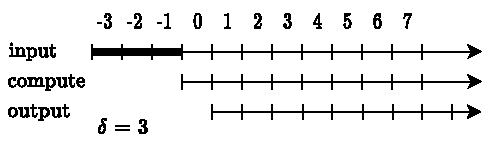
\includegraphics[width=0.75\linewidth]{Online_Timing.pdf}
    \caption{Timing characteristics of online operation with $\delta = 3$.}
    \label{fig:online_op}
\end{figure}

% Owing to this property, the intermediate results need not be stored, rather they are consumed in the successive computation, resulting in a decreased number of read/write operation from/to memory, hence low bandwidth requirements and consequent energy savings. In order to generate the output on the basis of partial input information, the online computation requires flexibility in computing digits. This is done by employing redundant digit number system. To this end, signed digit (SD) redundant number system in which number representation is done in radix ($r$) format is usually employed which has more than $r$ values for the representation of a given value. In this study, we use symmetric radix-$2$ redundant digit set of ${-1, 0, 1}$. For compatibility, the online modules use fractional numbers, this also simplifies the alignment of the operands. The first digit of the operand has weight of $r^{-1}$, and at a given iteration $j$, the digit $x_j$ is represented by two bits $x^+$ and $x^-$, and the numerical value is given by \eqref{eq: digit}.
The property of generating outputs based on partial input information in online computation negates the need to store intermediate results. Instead, these results are immediately consumed in subsequent computations. Consequently, this leads to a reduction in the number of read/write operations to memory, resulting in lower bandwidth requirements and subsequent energy savings.

To facilitate generating outputs based on partial input information, online computation relies on flexibility in computing digits. This is achieved by employing a redundant digit number system. In this study, a signed digit (SD) redundant number system is utilized, where numbers are represented in a radix-($r$) format that offers more than $r$ values for representing a given value. Specifically, a symmetric radix-$2$ redundant digit set of ${-1, 0, 1}$ is used. To ensure compatibility, the online modules work with fractional numbers, simplifying operand alignment. In this system, the first digit of the operand carries a weight of $r^{-1}$, and at a given iteration $j$, the digit $x_j$ is represented by two bits, namely $x^+$ and $x^-$. The numerical value of the digit is computed according to equation \eqref{eq: digit}.

\begin{equation} \label{eq: digit}
    x_j = SUB(x^+,x^-)
\end{equation}

% \paragraph{Input and Output}
The input and outputs are given as \eqref{eq: input} and \eqref{eq: output} respectively.
\begin{equation} \label{eq: input}
    x[j]= \sum_{i=1}^{j+\delta}x_{i}r^{-i}
\end{equation}
\begin{equation} \label{eq: output}
    z[j]= \sum_{i=1}^{j}z_{i}r^{-i},
\end{equation}
where $j$ represents the iteration index and the subscript $i$ denote the digit index. %A given online algorithm executes for $n+\delta$ cycles. The single digit input is fed for $n$ iterations, and after $\delta$ cycles a single output digit is generated in each iteration. 
In a given online algorithm, the execution spans $n+\delta$ cycles. The algorithm processes a single digit input for $n$ iterations. After $\delta$ cycles of providing the first input digit, it generates a single output digit in each subsequent iteration. This approach emphasizes digit-level processing and output generation, contributing to the overall efficiency of online computation.

\subsubsection{Online Multiplier (OLM)} \label{sec: Online_mult}
% In most CNN designs, the convolution during inference is carried out by multiplying a constant weight kernel with the input image in a sliding window fashion. This particular characteristic of CNNs suggests that the kernel matrix must be used multiple times for the convolution operation. In this context, an online multiplier, with one operand in parallel and the other in serial manner, can be useful, where the weight kernel can be employed in parallel and input can be fed in serial manner. In this study, we use the non-pipelined serial-parallel multiplier presented in \cite{usman2023low}, and depicted in the following Fig.~\ref{fig:mult_add}(a). The multiplier generates its output in MSDF fashion after an online delay of $\delta = 2$ cycles. The serial input and and output in each cycle are represented as \eqref{eq: input} and \eqref{eq: output} respectively, while the constant weight is represented as:
In most CNN designs, the convolution during inference involves multiplying a constant weight kernel with the input image in a sliding window fashion. This characteristic implies that the kernel matrix must be used multiple times for the convolution operation. In this context, an online multiplier with one operand in parallel and the other in a serial manner can be advantageous, allowing the weight kernel to be employed in parallel while the input is fed in a serial manner. In this study, a non-pipelined serial-parallel multiplier, as presented in \cite{usman2023low} and depicted in Fig.~\ref{fig:mult_add}(a), is used. The multiplier generates its output in a MSDF fashion after an online delay of $\delta = 2$ cycles. The serial input and output in each cycle are represented as \eqref{eq: input} and \eqref{eq: output}, respectively, while the constant weight is represented as:
\begin{equation}
    Y[j] = Y = -y_0 \cdot r^0 + \sum_{i=1}^{n} y_ir^{-i}
 \end{equation}
% Further derivations related to the recurrence and selection function of the serial-parallel online multiplier can be found in \cite{usman2023low}.
Additional details related to the recurrence stage and selection function of the serial-parallel online multiplier are available in \cite{usman2023low}.
% \begin{figure}[htb]
%     \centering
%     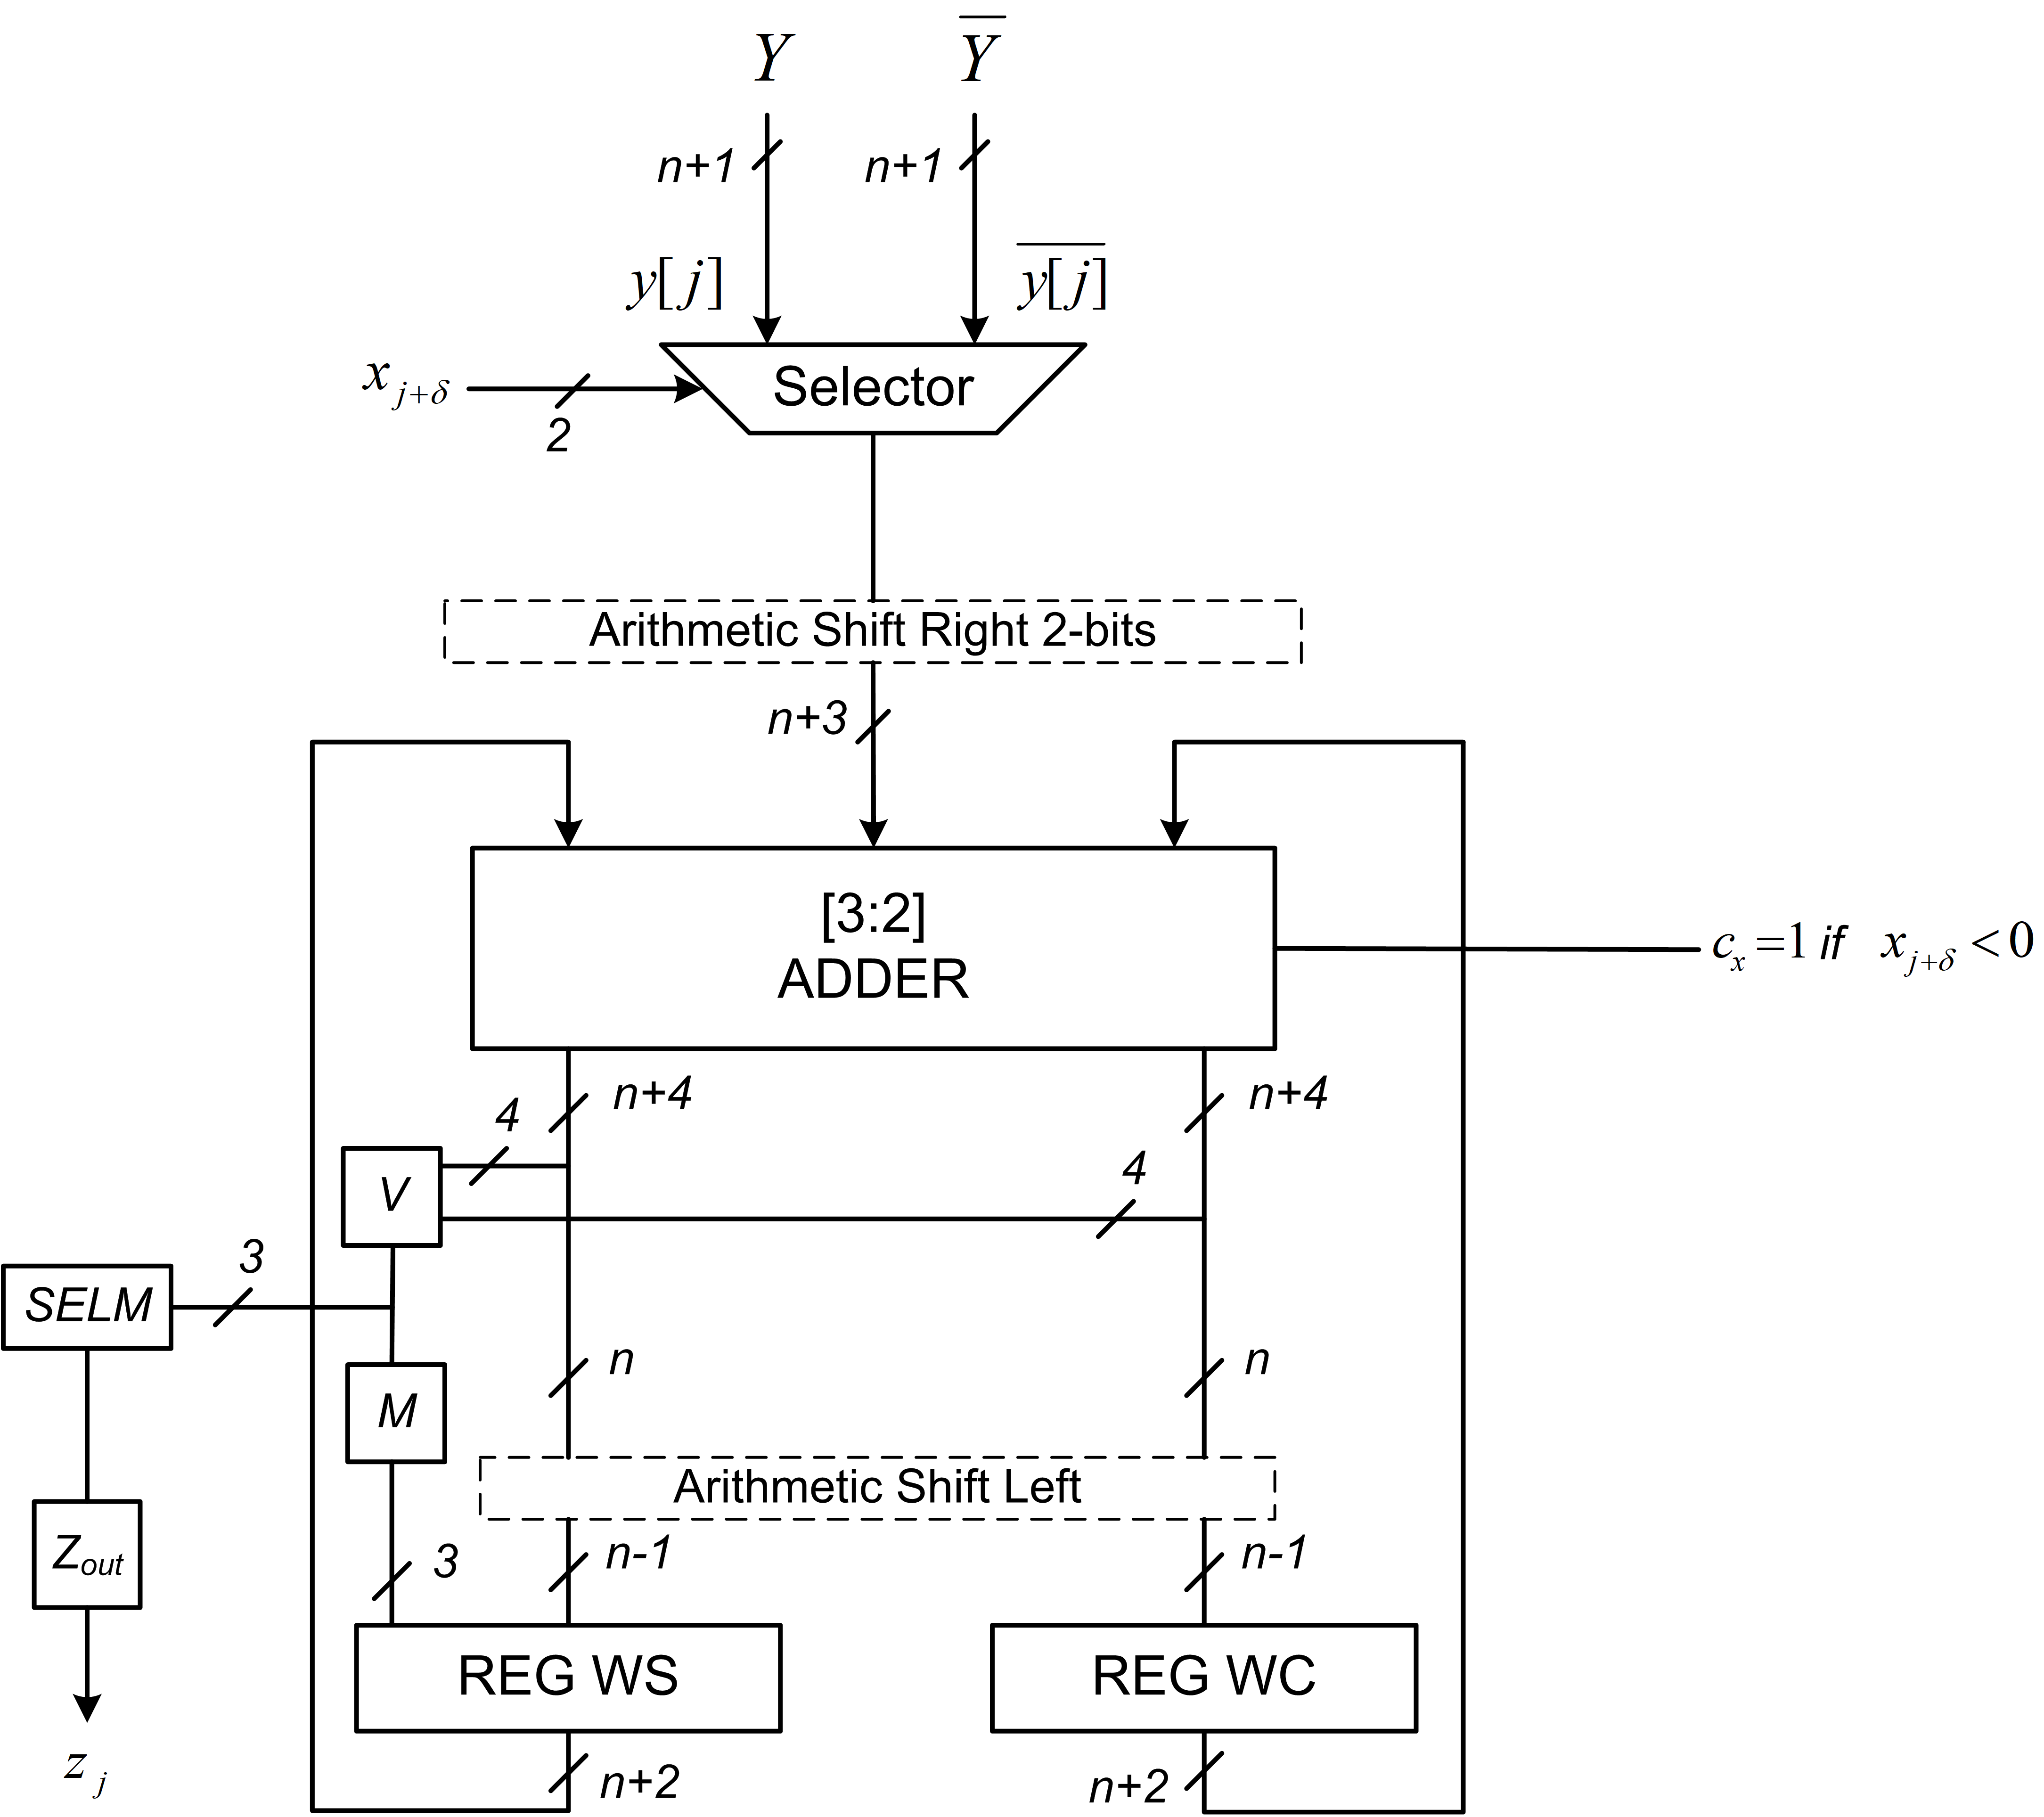
\includegraphics[width=\linewidth]{Serial_Parallel.png}
%     \caption{Online Serial-Parallel Multiplier \cite{usman2023low}}
%     \label{fig:ser_par}
% \end{figure}

\subsubsection{Online Adder (OLA)} \label{sec: Online_adder}
% Since the multipliers used in this study generate their outputs in an MSDF fashion, an adder with similar capability is needed to compute the sum-of-product (SOP). In this context, a digit-serial online adder that takes both its inputs and generates its output in an MSDF fashion, is employed. This enables digit-level pipelining in the proposed SOP design and also helps in the early determination and subsequently termination of negative activations. The online adder with an online delay of $\delta = 2$, follows a simple construction as presented in Fig.~\ref{fig:mult_add}(b).
As the multipliers utilized in this study produce outputs in an MSDF fashion, an adder with a similar capability is essential for computing the SOP. In this context, a digit-serial online adder, which takes both inputs and generates its output in an MSDF fashion, is employed. This choice facilitates digit-level pipelining in the proposed SOP design and contributes to the early detection and subsequent termination of negative activations. The online adder, with an online delay of $\delta = 2$, follows a straightforward construction, as illustrated in Fig.~\ref{fig:mult_add}(b).
% Similar to the multiplier presented in the previous section, the online adder also generates its output in an MSDF manner after $\delta = 2$ cycles. 
Further details and relevant derivations can be found in \cite{ercegovac2004digital}.
% \begin{figure}[htb]
%     \centering
%     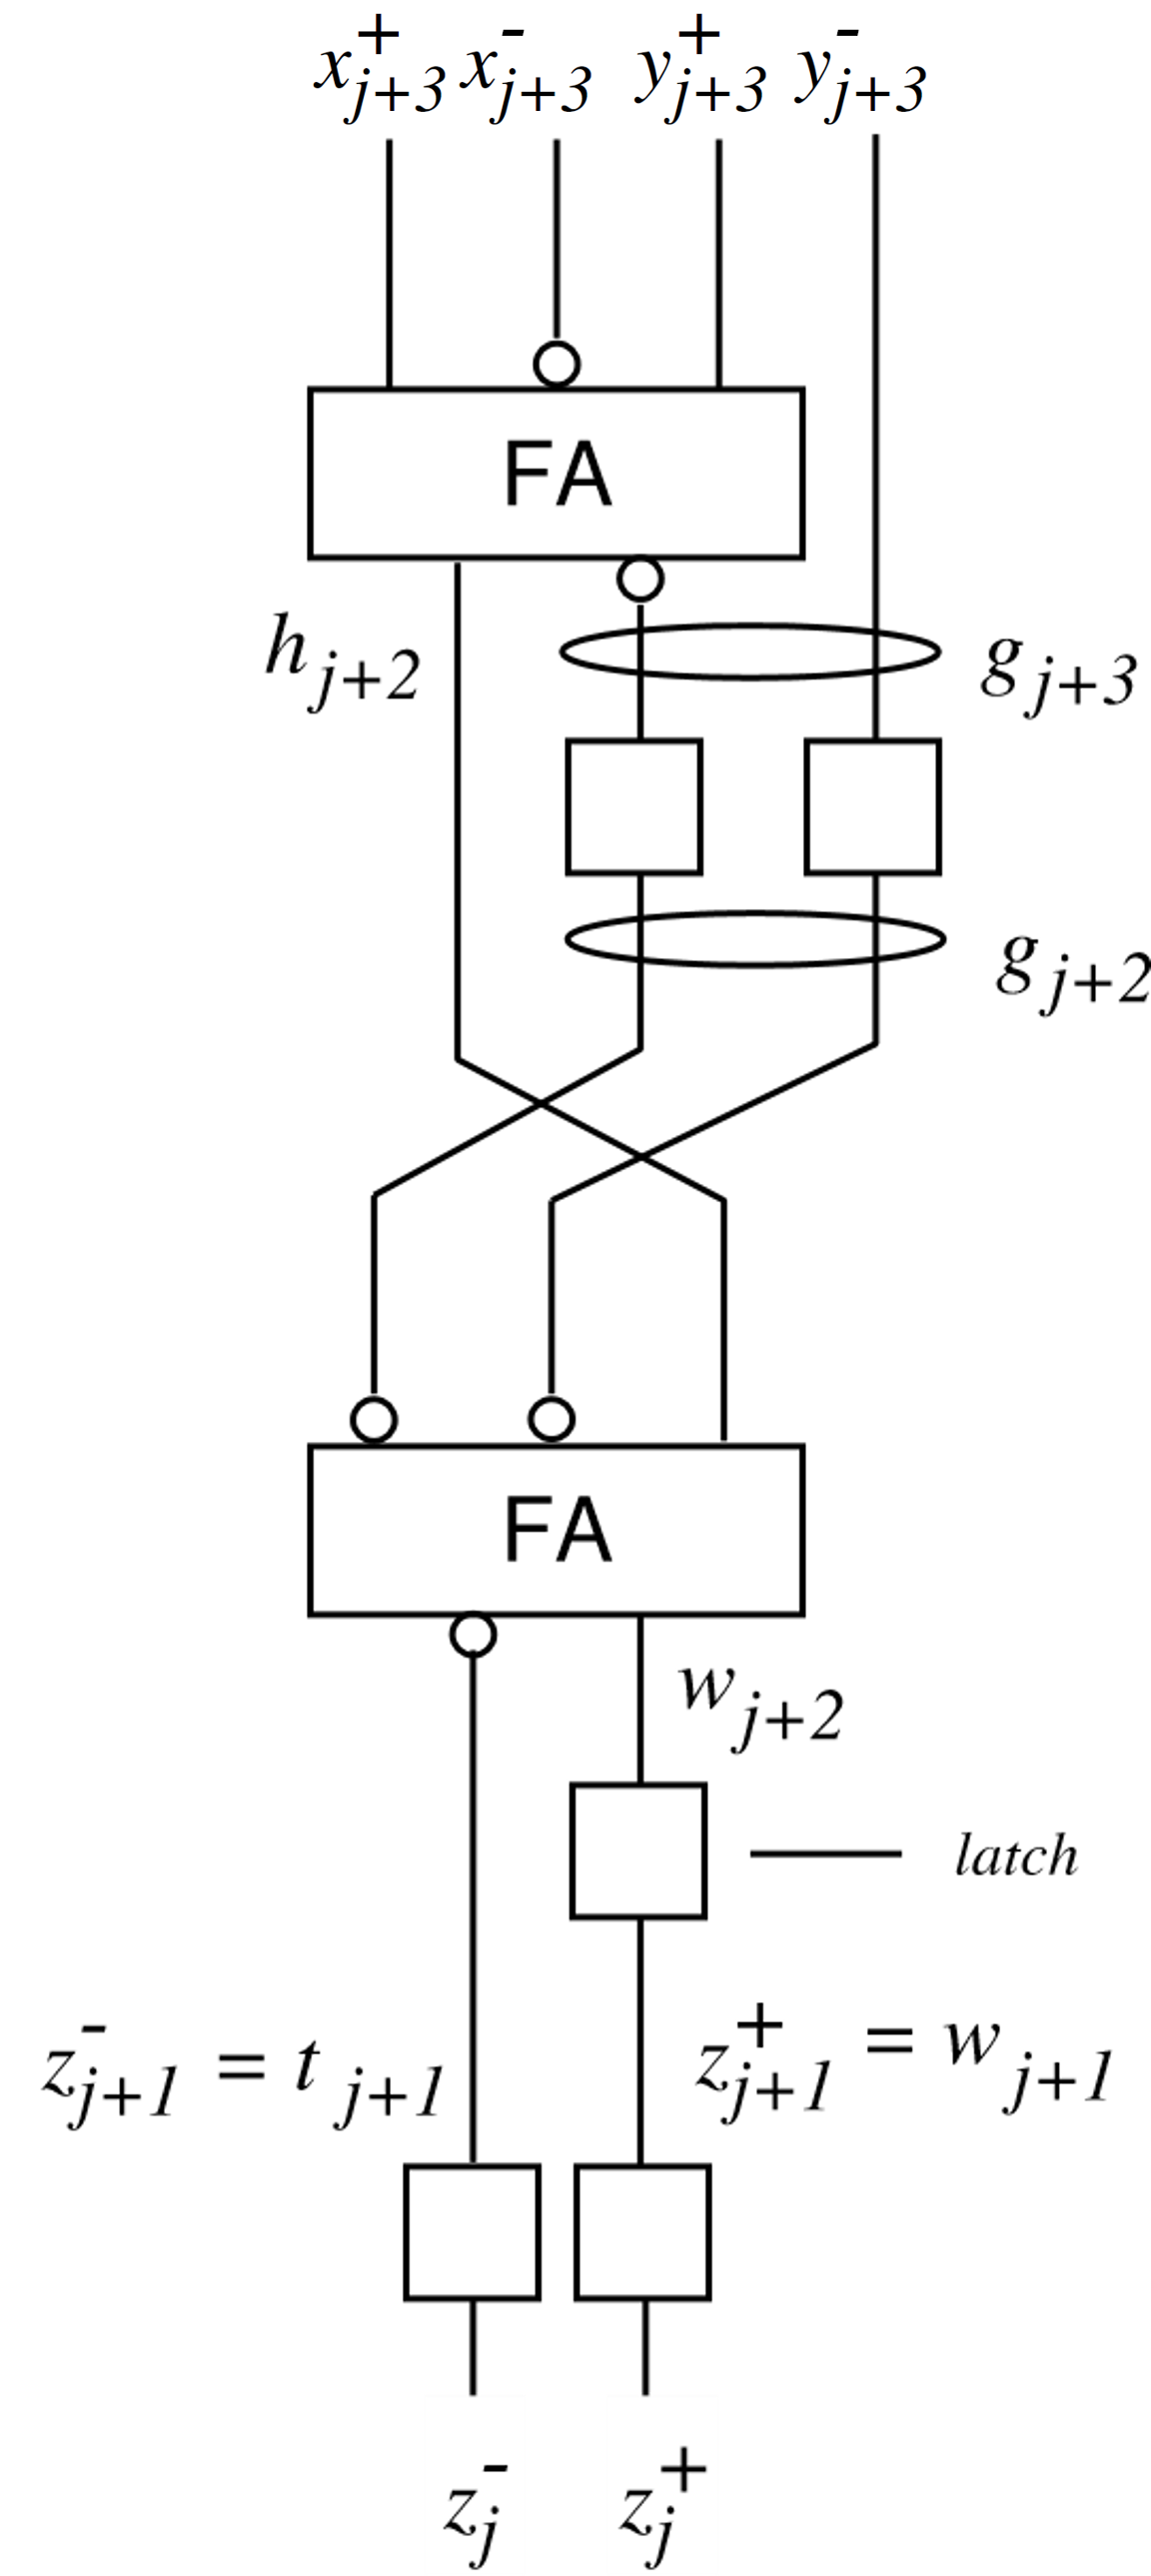
\includegraphics[width=0.3\linewidth]{online_adder.png}
%     \caption{Online Adder \cite{ercegovac2004digital}}
%     \label{fig:online_adder}
% \end{figure}

\begin{figure}[!htb]
    \centering
    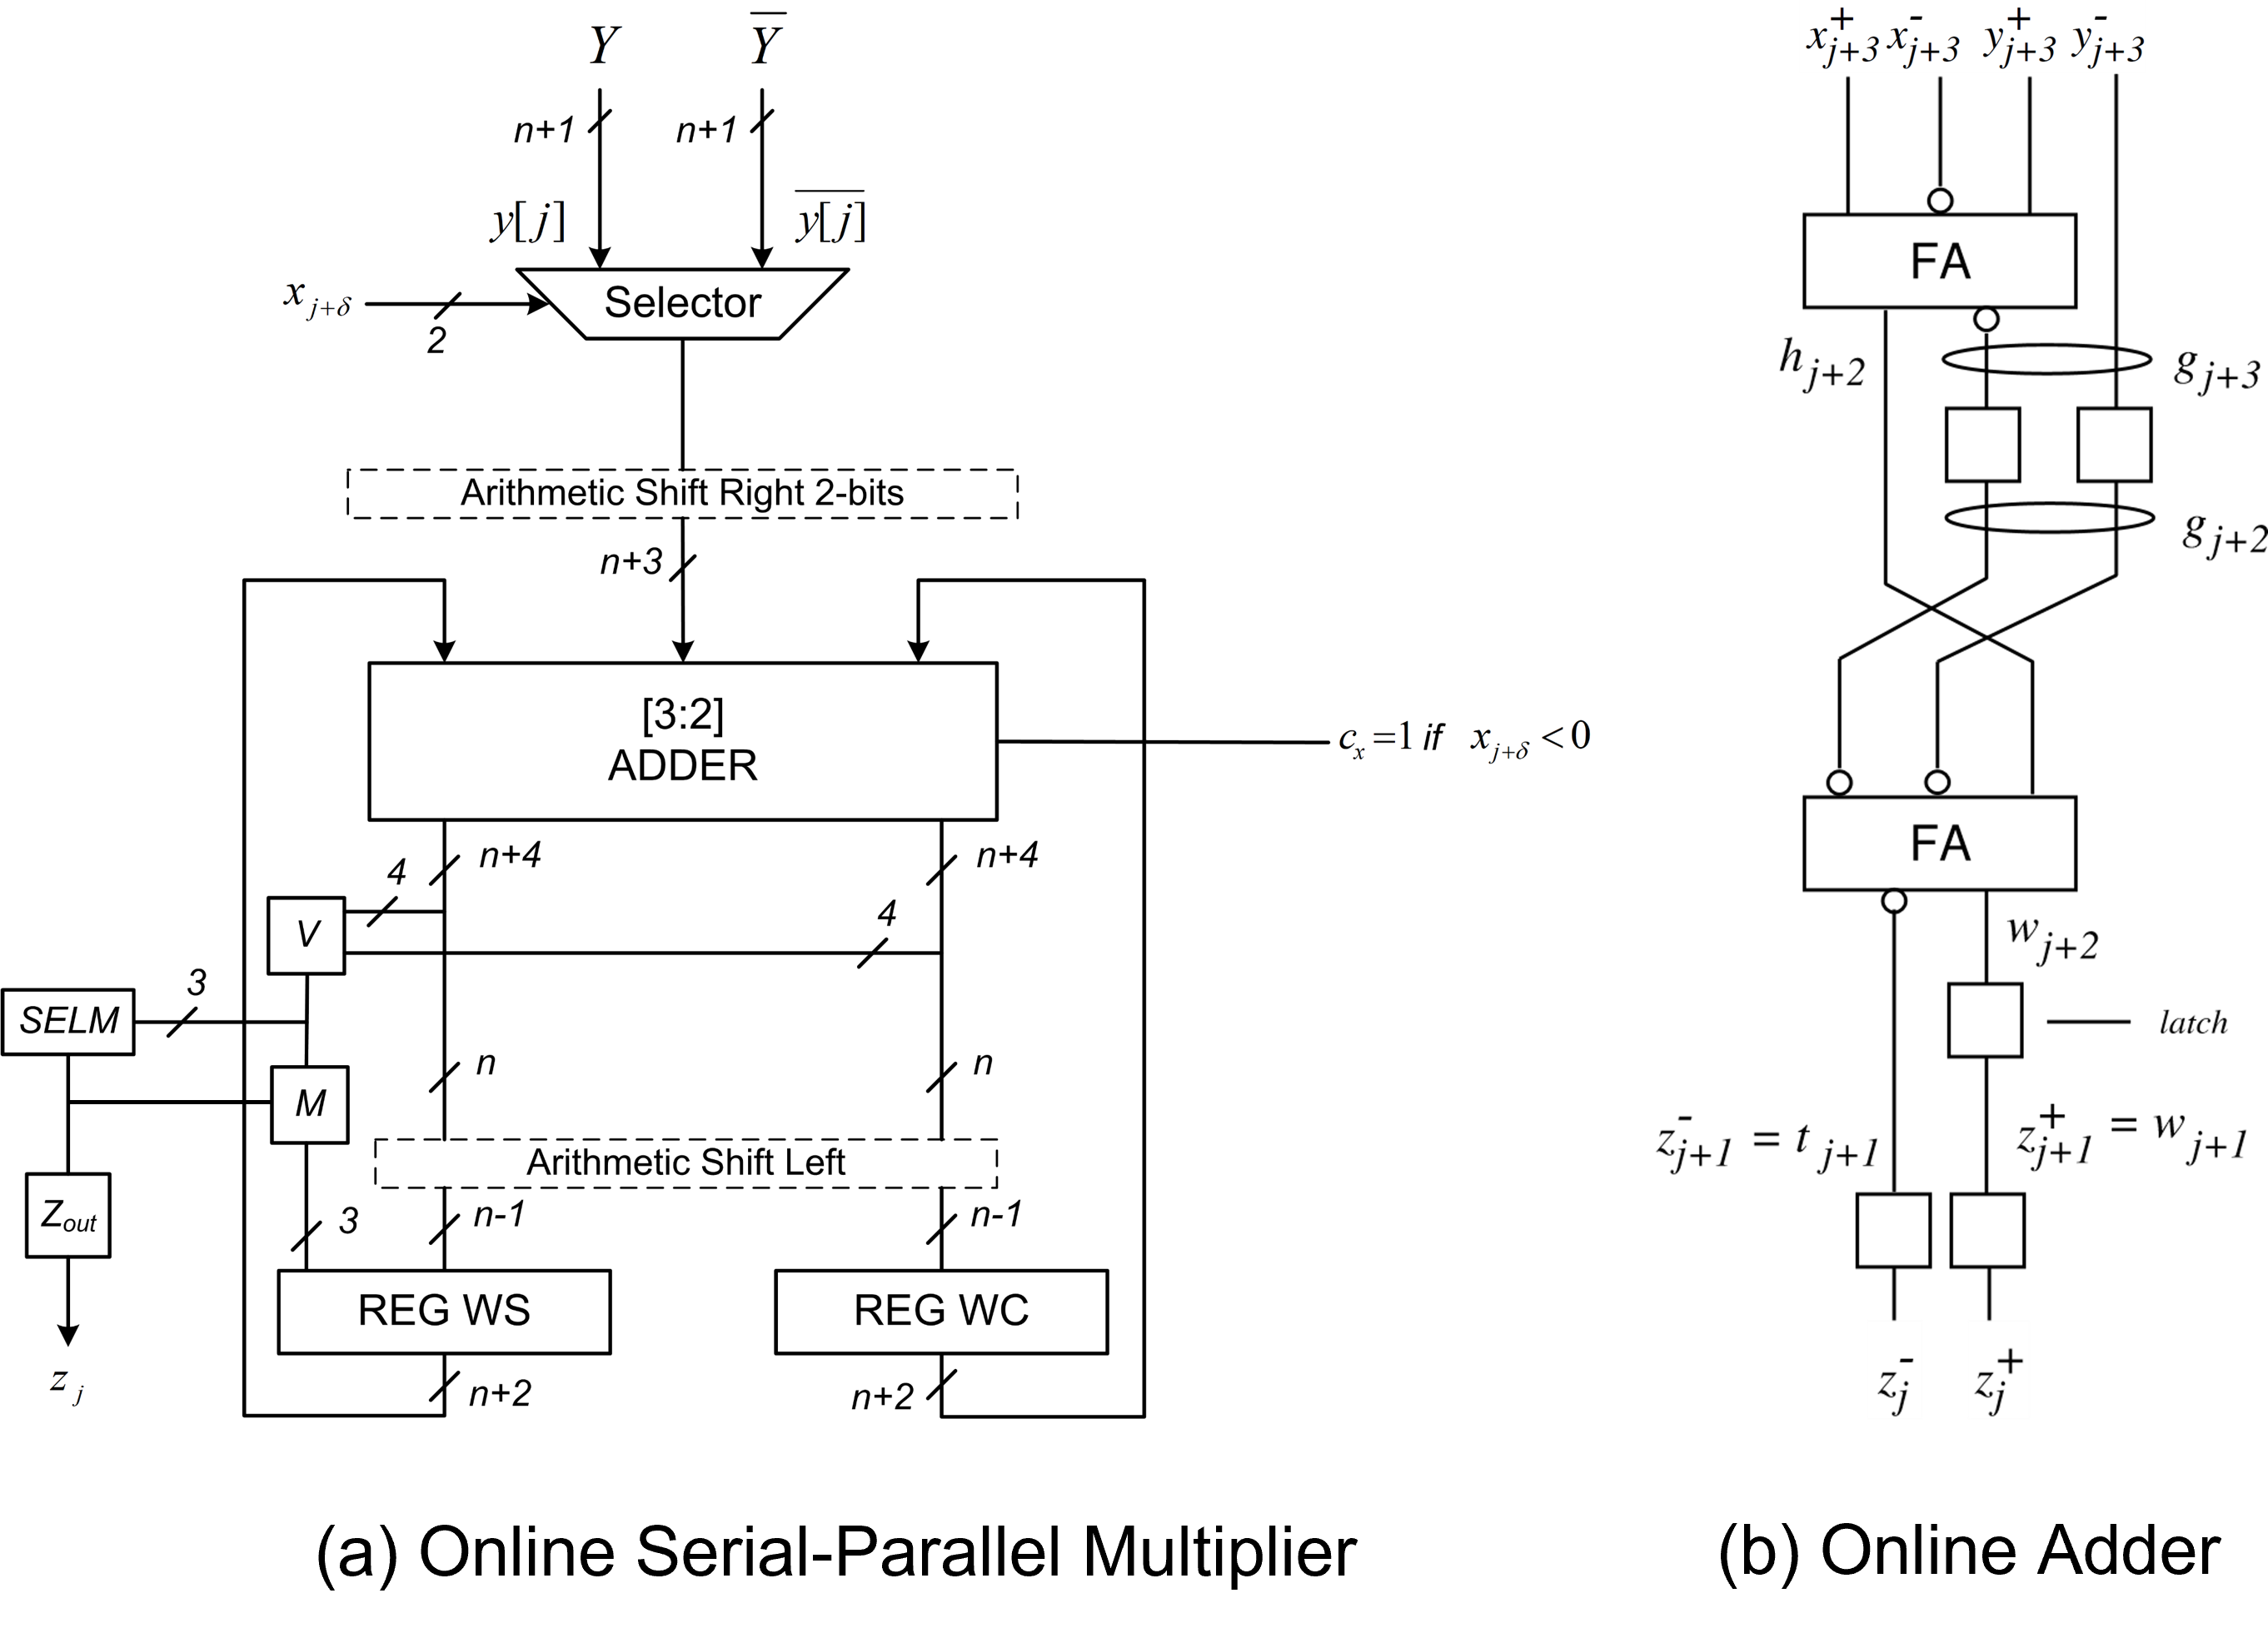
\includegraphics[width=\linewidth]{mult_add.png}
    \caption{Basic Components (a) Online Serial-Parallel Multiplier \cite{usman2023low}, where $x$ is the serial input and $Y$ is the parallel output, (b) Online Adder \cite{ercegovac2004digital}}
    \label{fig:mult_add}
\end{figure}


\subsection{Proposed Design} %\textcolor{red}{START HERE}
% This section details the architecture of the proposed DSLOT-NN based on online computation units with early termination capability. The arrangement of computation units in the processing engine (PE) of DSLOT-NN and the techniques for terminating ineffectual convolutions (resulting as negative) are discussed.
This section provides a detailed overview of the architecture of the proposed design, which is built upon online computation units featuring early detection and termination capabilities for negative outputs. The arrangement of computation units within the processing engine (PE) of the proposed design, along with the techniques for identifying and terminating ineffective convolutions (resulting in negative outputs), is thoroughly discussed.

\subsubsection{Processing Engine Architecture}
% The architecture of the proposed DSLOT-NN is presented in Fig.~\ref{fig:Proposed}. Each PE, presented in Fig.~\ref{fig:PE} contains $k \times k$ online serial-parallel multipliers followed by a reduction tree to generate one output pixel. The input pixel is fed serially while the kernel pixel is fed in parallel, depicted by the thickness of the arrows in Fig.~\ref{fig:Proposed}. The arrangement of PEs is done in such a way that the outputs of the $4$ PEs will directly be fed to the ensuing pooling layer. It is worth noting that the architecture presented in Fig.~\ref{fig:Proposed} is designed for a CNN with single input feature map. A similar approach can be followed for a CNN with multiple input feature maps. A generic representation of the DSLOT-NN is also presented in the following sections.

Each processing engine (PE), as illustrated in Fig.~\ref{fig:PE}, is equipped with $K \times K$ online serial-parallel multipliers, succeeded by a reduction tree comprising online adders. This configuration is designed to compute a $K \times K$ convolution on an input channel or feature map. The input pixel is serially fed in a digit-by-digit manner, while the kernel pixel is concurrently fed in parallel, as indicated by the thickness of the arrows in Fig.~\ref{fig:PE}.

\begin{figure}[!htb]
    \centering
    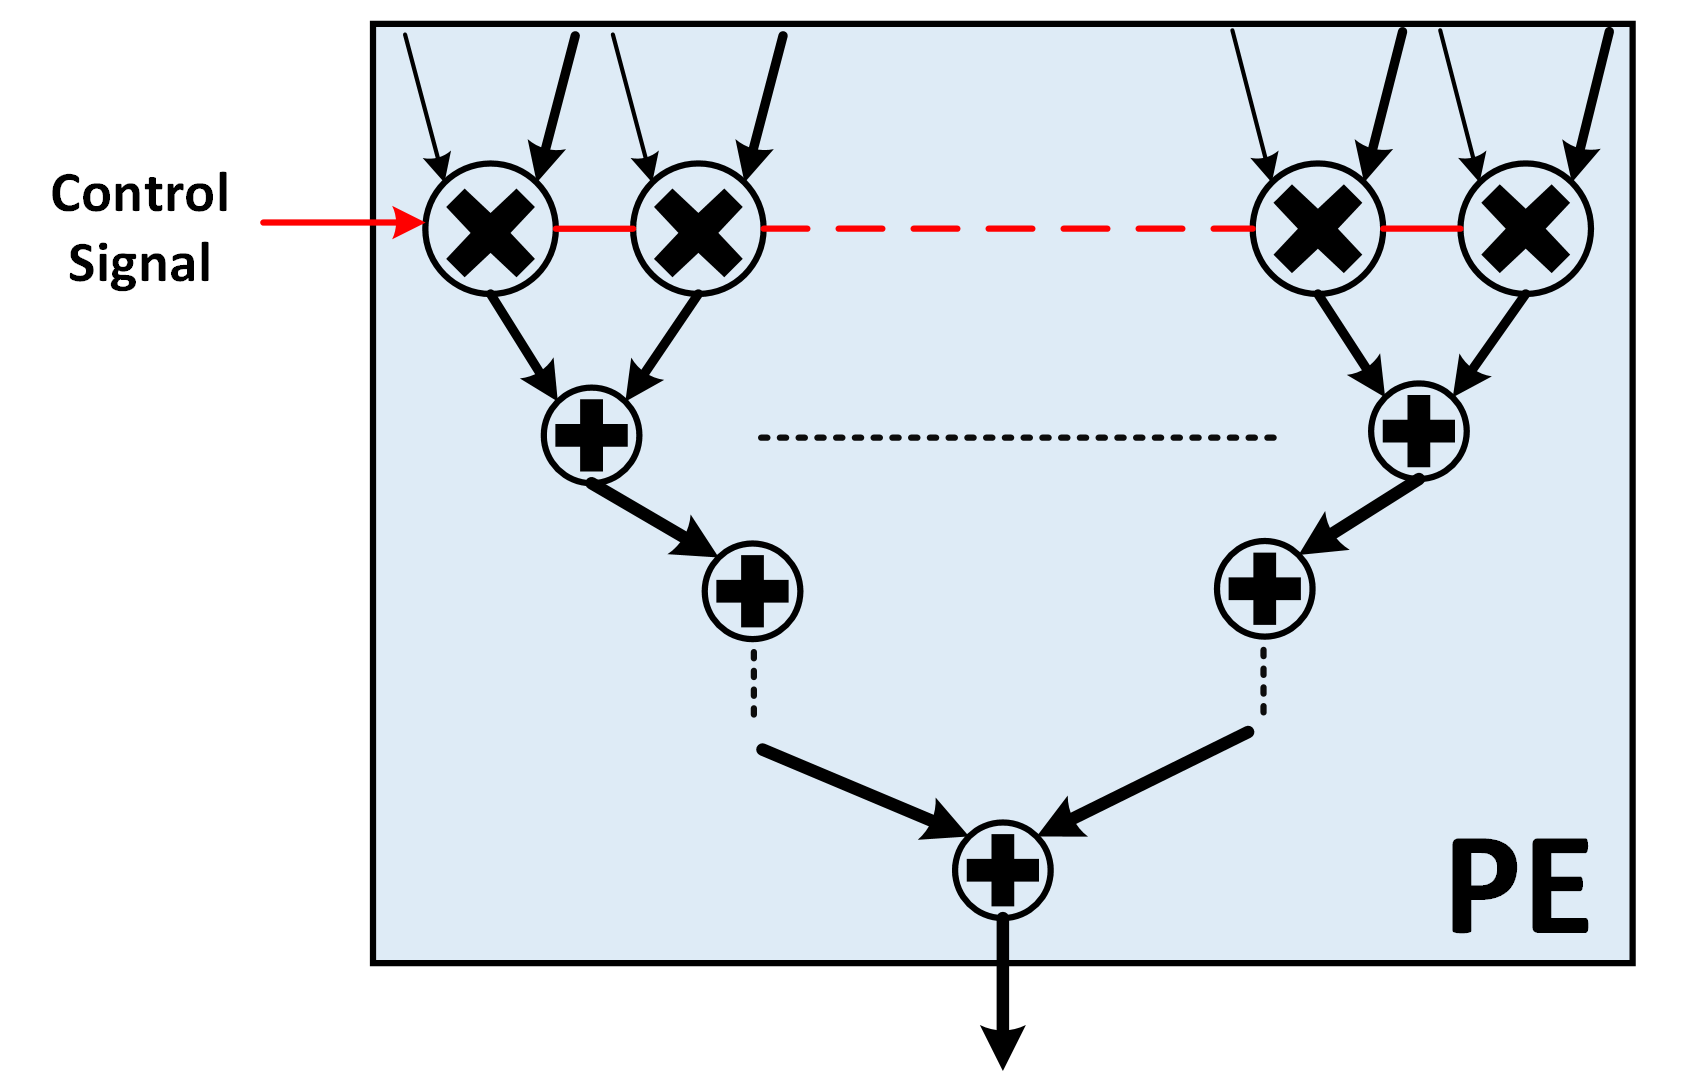
\includegraphics[width=0.9\linewidth]{PE.png}
    \caption{Processing engine architecture of the proposed design. Each PE contains $K\times K$ multipliers where each multiplier accepts a bit-serial (input feature) and a parallel (kernel pixel) input.}
    \label{fig:PE}
\end{figure}

% \begin{figure*}[!htb]
%     \centering
%     \includegraphics[width=0.75\linewidth]{Proposed_design.png}
%     \caption{DSLOT-NN block diagram}
%     \label{fig:Proposed}
% \end{figure*}

 
Each multiplier in the PE is responsible for the multiplication of one pixel in the convolution window with the corresponding pixel in the same feature map of the convolution kernel. Therefore, all the $(K \times K)$ pixels are processed in parallel. The number of cycles required for a PE to generate its output can be calculated as follows

% \begin{equation} \label{eq: num_cycles}
%     \begin{split}
%         Num_{Cycles} = \delta_{Mult} + \delta_{Add} \times \ceil{log_{2}(K \times K)} + \\
%         \delta_{+} \times \ceil{log_{2}(N)} + p_{out}
%     \end{split}
% \end{equation}
\begin{equation} \label{eq: num_cycles}
    % \begin{split}
        PE_{Cycles} = \delta_{Mult} + \delta_{Add} \times \ceil{log_{2}(K \times K)} + p^{PE}_{out}
    % \end{split}
\end{equation}
where $\delta_{Mult}$ and $\delta_{Add}$ are the online delays of online multiplier and adder respectively, $\ceil{log_{2}(K \times K)}$ is the number of reduction tree stages required to generate the SOP of the $K \times K$ multipliers, 
% $\ceil{log_{2}(N)}$ is the number of reduction tree stages required to add the SOP results of $N$ input feature maps, 
and $p^{PE}_{out}$ is the precision of the SOP result generated by a PE. $p^{PE}_{out}$ is calculated as follows.
\begin{equation} \label{eq:pout}
     p^{PE}_{out} = p_{out}^{Mult} + \ceil{log_{2}(k \times k)}
\end{equation}

% Each adder in the following reduction tree also processes the inputs in a digit serial fashion and generates most-significant output digits first. The online delay of the Similar to the multiplier, the adders also generate the output digits after a negligible initial delay.
% , which are collected by the adders in the next stage of the reduction tree.

% \begin{figure}[htb]
%     \centering
%     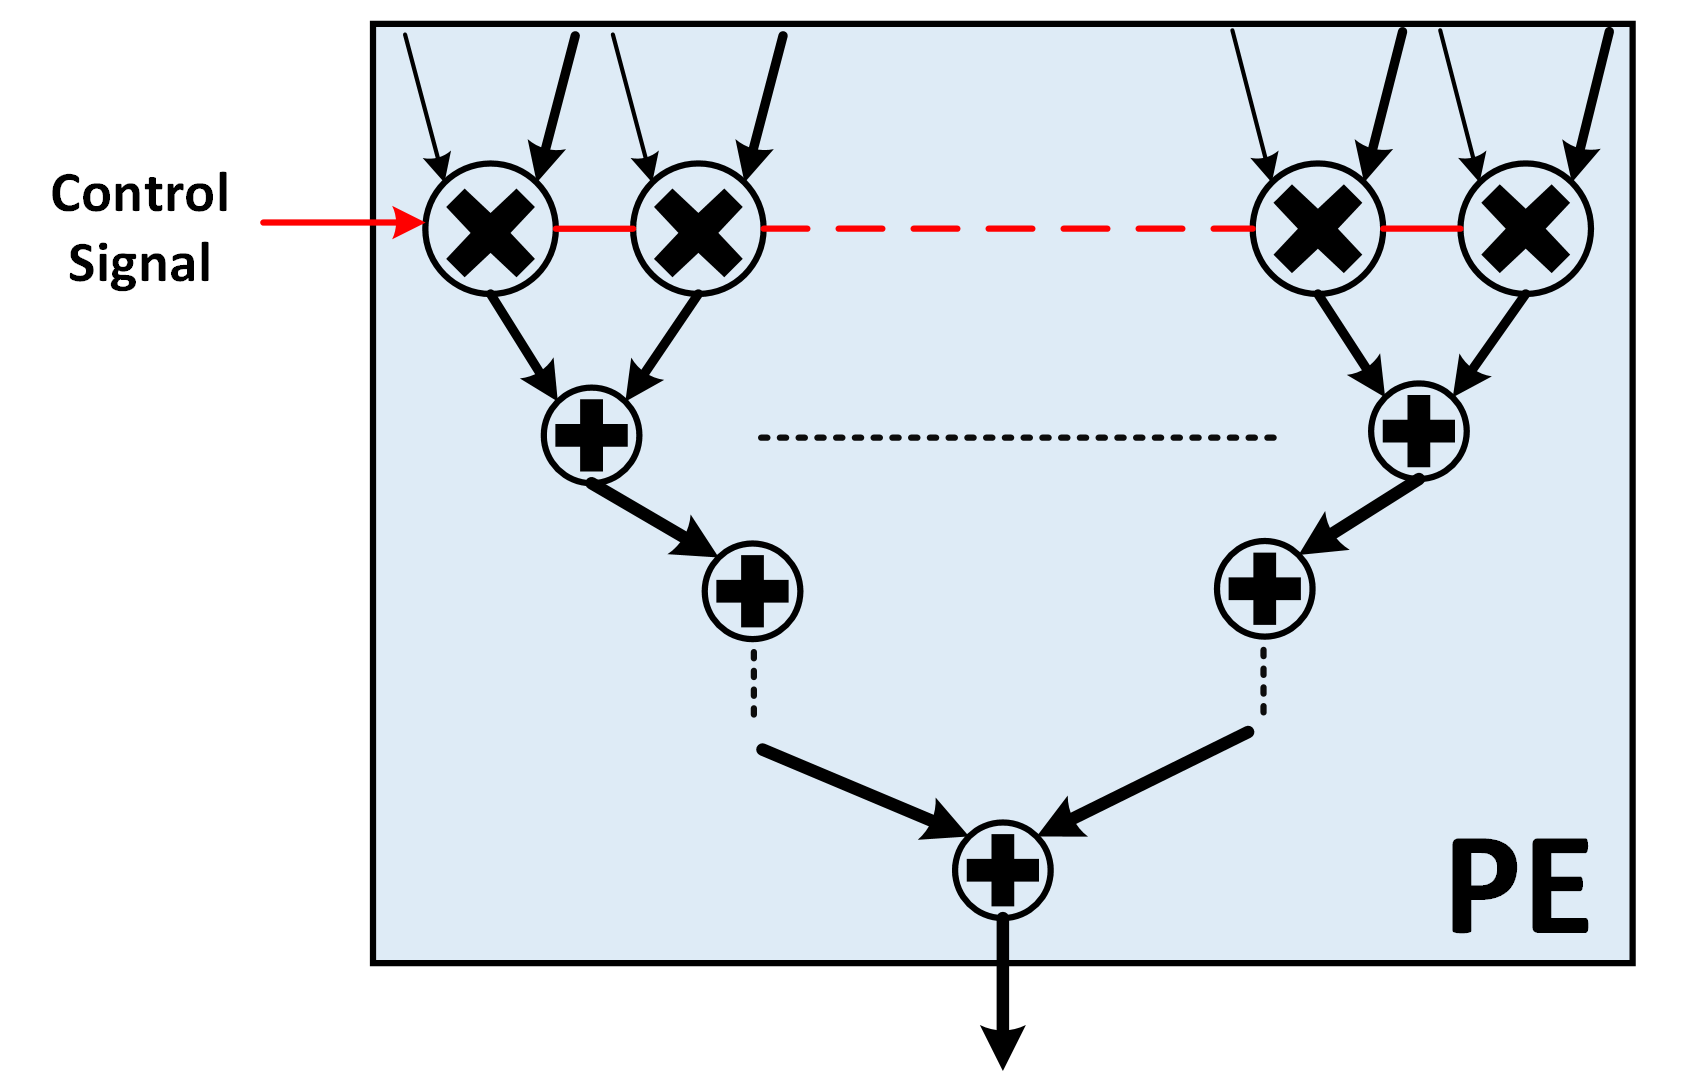
\includegraphics[width=0.85\linewidth]{PE.png}
%     \caption{Processing Element Architecture}
%     \label{fig:PPE}
% \end{figure}

\subsubsection{Early Detection and Termination of Negative Computations}
% Most CNN accelerator designs put emphasis on the faster or efficient generation of the sum-of-product (SOP), but only a few works discuss the possibility of early assessment of negative values for the activation layer (ReLU). The early determination of negative activations is a challenging problem in accelerators based on conventional arithmetic. For instance, the bit-serial multipliers takes \emph{multiplicand} in parallel and the \emph{multiplier} is processed serially. In each iteration a partial product is generated and stored in register, which is then shifted into appropriate positions before being added to other partial products to obtain the final product. Typically a series of adders, such as carry save adders, ripple-carry adders, etc., are employed to perform this reduction. In convolution, another level of reduction is required to get the output pixel. Furthermore, another level of reduction is needed, if there are more than $1$ input feature maps, to compute the SOP. In conventional bit-serial multipliers, the determination of the most significant bit and the identification of the result's polarity require waiting until all partial products have been generated and added to the previous partial sums. Among the few works that aim to solve the early detection of the negative activations, use either a digit encoding scheme or an estimation technique for early negative detection \cite{lee2018compend, chen2019comprrae, kim2021compreend}.

% Since every accelerator design uses some kind of MAC operations where the final output of convolution results as the output of an adder tree or accumulator where the final result MSDs depend highly on the carry propagation from the digits of lower weights, therefore, the widely used arithmetic and digit encoding schemes have an inherent reliance on the carry propagation which hinders the ability to perform early detection of negative values.

% due to the very reason that most accelerator architectures use conventional parallel arithmetic units or conventional digit-serial arithmetic units i.e. multipliers, adders, MACs, accumulators, etc. 

In most designs of CNN accelerators, the focus is often on achieving faster and more efficient generation of the SOP. However, only a limited number of works explore the potential for early assessment of negative values in the activation layer, particularly for ReLU. Early detection, and the subsequent termination of computation, of negative activations poses a significant challenge in accelerators based on conventional arithmetic. For example, in bit-serial multipliers, the \emph{multiplicand} is processed in parallel, while the \emph{multiplier} is processed serially. In each iteration, a partial product is generated and stored in a register. This partial product is then shifted into appropriate positions before being added to other partial products to obtain the final product. Typically, a series of adders, such as carry-save adders or ripple-carry adders, is employed to perform this reduction. In the case of convolution, an additional level of reduction is required to obtain the output pixel. Moreover, if there are more than one input feature maps, another level of reduction is needed to compute the SOP. In conventional bit-serial multipliers, determining the most significant bit and identifying the polarity of the result requires waiting until all partial products have been generated and added to the previous partial sums. Among the limited works addressing the early detection of negative activations, some utilize either a digit encoding scheme or an estimation technique for early negative detection \cite{kim2021compreend}, while others focus on complex circuit designs \cite{shuvo2020msb}.

% The challenge of early detection and termination of negative activations can be addressed by the intrinsic ability of online arithmetic to generate output digits in an MSDF manner. The proposed design supports the termination of negative activation computation in $p$ cycles, where $p< \mathbb{N}$, and $\mathbb{N}$ is the number of cycles to compute complete result. This is done by observing and comparing the output digits. The process of detecting the negative activations and subsequently terminating the relevant computation is summarized in Algorithm \ref{alg:ENT}.

The challenge of early detection and termination of negative activations can be effectively addressed by leveraging the inherent capability of online arithmetic to generate output digits in a MSDF manner. The proposed design facilitates the detection and the subsequent termination of negative activation computation within \(p\) cycles, where \(p < \mathbb{N}\) and \(\mathbb{N}\) represents the number of cycles needed to compute the complete result. This is achieved by monitoring and comparing the output digits. The process of detecting negative activations and subsequently terminating the relevant computation is outlined in Algorithm \ref{alg:ENT}.


\begin{algorithm}[!ht]
\caption{Early detection and termination of negative activations}\label{alg:ENT}
\begin{algorithmic}[1]
\State $z^{+}[j],\ z^{-}[j] $ \texttt{bits}\;
\For{\texttt{j : 1 \ to \ $Num_{Cycles}$}}
    \State $z^{+}[j] \gets Concat(z^{+}[j] \ , \ z^{+}_{j})$\;
    \State $z^{-}[j] \gets  Concat(z^{-}[j] \ , \ z^{-}_{j})$\;
    \If{$z^{+}[j] < z^{-}[j]$}
        \State \texttt{Terminate}
    \Else
        \State \texttt{Continue}
    \EndIf
\EndFor
\end{algorithmic}
\end{algorithm}


% The ReLU unit is equipped with registers to store redundant output $z^{+}[j]$ and $z^{-}[j]$ bits, which are the positive and negative output digits of the SOP representing the output SOP in redundant number representation. During each iteration, the new digits are concatenated, indicated by "$\frown$" in Algorithm \ref{alg:ENT}, with their corresponding previous digits and as soon as the value of $z^{+}[j]$ goes below the value of $z^{-}[j]$ indicating a negative output, a termination signal is generated by the control unit and the computation of the SOP is terminated. Fig.~\ref{fig:Proposed}, shows the block diagram of the proposed DSLOT-NN considering one input feature map. This simple procedure of early negative detection can save upto $45 - 50\%$ of the computation cycles for a convolution operation resulting in a negative number subsequently resulting in an energy efficient design. According to \eqref{eq: num_cycles}, the number of cycles required by the proposed design to process one convolution is found to be $33$, where $\delta_{\times} = \delta_{+} =2$, $k=5$, $N=1$, and $p_{out} = 21$ considering the bit growth in the reduction tree stages. 
% Where $p_{out}$ is calculated by eq. \ref{eq:pout} as,  $p_{out}^{Mult} = 16$ and $\ceil{log_{2}(k \times k)} = 5$, with $k \times k  = 5 \times 5 = 25$ as the convolution kernel dimensions.
The ReLU unit is equipped with registers to store the output \(z^{+}[j]\) and \(z^{-}[j]\) bits, representing the positive and negative output digits of the SOP in redundant number representation. During each iteration, the new digits are concatenated, as indicated in Algorithm \ref{alg:ENT}, with their corresponding previous digits. As soon as the value of \(z^{+}[j]\) drops below the value of \(z^{-}[j]\), indicating a negative output, a termination signal is generated by the control unit, and the computation of the relevant SOP is terminated. This simple procedure, aided by the inherent properties of online arithmetic, of early detection and termination of negative outputs can save a significant number of computation cycles required for a convolution operation resulting in a negative number, leading to substantial energy savings.

\subsubsection{Proposed Accelerator Design}
% A general extension of the proposed DSLOT-NN for larger networks is presented in Fig.~\ref{fig:DSLOT}. The number of PEs in a processing block (PB) depend upon the number of input feature maps for a particular convolution layer in a CNN. This generic architecture can be repeated multiple times depending upon the number of output feature maps if more parallelism is required. 

% The PBs are responsible for the computation of one of the pixels belonging to a pooling (or maxpooling) window. In Fig.~\ref{fig:DSLOT}, we presented an example of a $2 \times 2$ pool window hence the 4 PBs. Each PB consists of multiple PEs followed by an online adder tree. The number of PEs in a PB represents the input tiling and it has a range of $(1, N)$, where $N$ is the number of input feature maps. The output digits of the adder tree are forwarded to a simple comparator circuit to perform the detection of negative activations for ReLU. The structure of a PE is presented in Fig.~\ref{fig:PE}.

\begin{figure}[!ht]
    \centering
    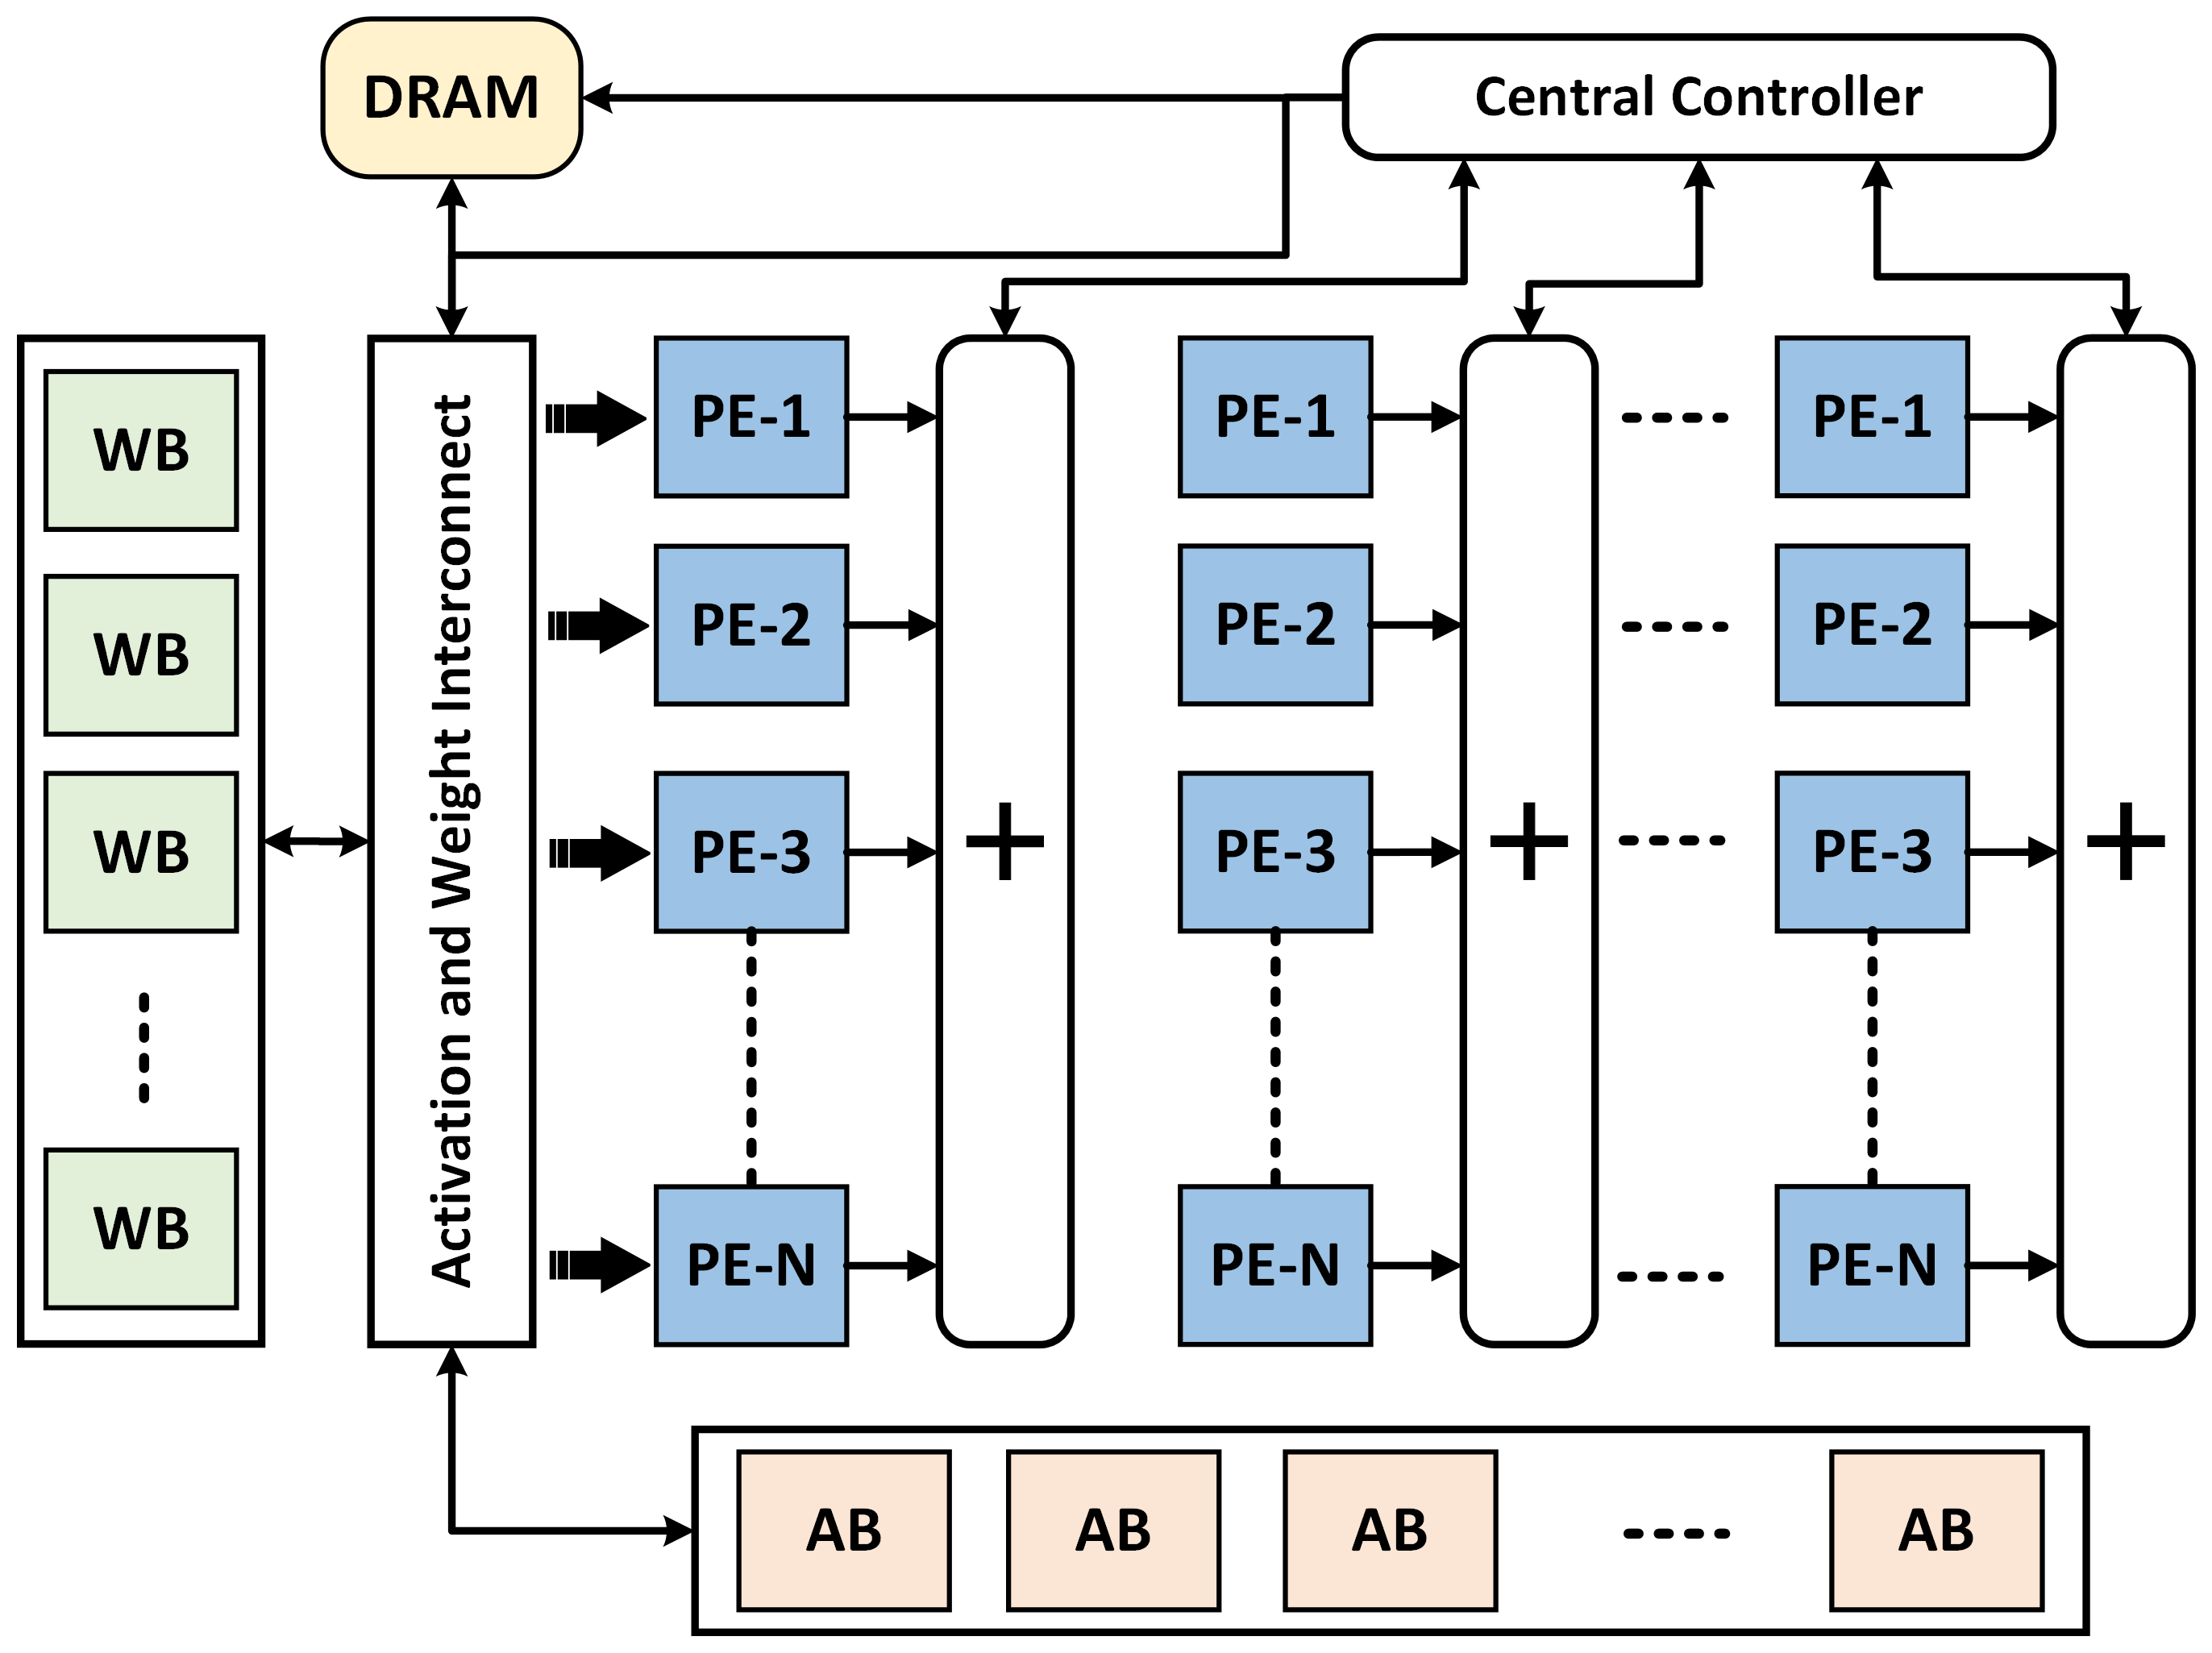
\includegraphics[width=\linewidth]{DSLOT_extension_Arch.png}
    \caption{Architecture of the proposed design for a convolution layer. Each column is equipped with \(N\) PEs to facilitate the input channels, while each column of PE is followed by an online arithmetic-based reduction tree for the generation of the final SOP. The central controller block generates the termination signals and also controls the dataflow to and from the weight buffers (WB) and activation buffers (AB).}
    \label{fig:DSLOT}
\end{figure}

The overall architecture of the proposed design is depicted in Fig.~\ref{fig:DSLOT}. It consists of multiple PEs arranged in a 2D array, where each column in the array contains \(N\) PEs. The outputs of these \(N\) PEs is forwarded to a reduction tree designed using online adders. The output digits from the reduction tree are forwarded to a ReLU decision block within the reduction tree where the polarity of the output activation is dynamically determined. If the output digit is determined to be negative, a termination signal is generated which is propagated to the central controller resulting in the subsequent termination of the computation in that column. By design, the proposed accelerator architecture supports input tiling by the invocation of \(N\) PE in each column. However, the number of columns in the accelerator array can be determined on the basis of the architecture of the CNN and the target hardware. The number of cycles required to generate the result of a convolution can be calculated as

\begin{equation} \label{eq: cyc_SOP}
    \begin{split}
        SOP_{Cycles} = \delta_{Mult} + \delta_{Add} \times \ceil{log_{2}(K \times K)} + \\
        \delta_{+} \times \ceil{log_{2}(N)} + p_{out}
    \end{split}
\end{equation}
Where \(\ceil{log_{2}(N)}\) is the number of reduction tree stages required to add the SOP results of $N$ input feature maps to generate the final output of the convolution. \(p_{out} = p^{PE}_{out} + \ceil{log_{2}(N)}\) is the precision of the final SOP result of the convolution.

At the end of each convolution SOP computation, the central controller generates signals for new input activations and/or weights to be loaded into the activation and weight buffers respectively. Moreover, it also generates the signals that direct the activations and weights from their respective buffers into the registers in the PEs. For a given convolution layer in a CNN, the central controller can also deactivate the PEs in a column and route the respective partial results directly to the reduction tree in that column. This can be done in resource constrained situations such as in edge devices where the compute resources are scarce. For instance, on such platforms, a large number of input channels \(N\) for a particular convolution layer can be implemented by reducing the number of PEs in a column and storing the results in the activation buffers. Upon completion of the computation of these \(N\) channels, the PEs of a column can be deactivated and the partial results can be added to determine the final SOP result. 

The convolution kernels and input activations stored in the DRAM, are pre-loaded into the weight buffers (WB) and activation buffers (AB) using the activation and weight interconnect. The activations and weights are then forwarded via the same interconnect to the PE array for computation. The results of the computations can either be written back to the DRAM or forwarded to the activation buffers depending upon the CNN layer configurations.

% The quantity of the PEs within a processing block (PB) is contingent on the number of input feature maps for a specific convolution layer in a CNN. This generic architecture can be replicated multiple times based on the number of output feature maps, allowing for increased parallelism as needed.

% The PBs are tasked with computing one of the pixels within a pooling (or max-pooling) window. In Fig.~\ref{fig:DSLOT}, we illustrate an instance of a $2 \times 2$ pool window, hence the presence of four PBs. Each PB is composed of multiple PEs followed by an online adder tree. The number of PEs in a PB denotes the input tiling and ranges from 1 to \(N\), where \(N\) represents the number of input feature maps. The output digits from the adder tree are directed to a simple comparator circuit to detect negative activations for ReLU activation block equipped with the proposed strategy of early detection and termination of negative outputs. The structure of a PE is outlined in Fig.~\ref{fig:PE}.





% Section~\ref{sec: Results} contains further details on the experiments conducted to determine the amount of clock cycles and the subsequent energy savings achieved due to the early detection and the termination of the negative activations.
The following section~\ref{sec: Results} contains details on the experiments conducted to ascertain the performance of the proposed design on modern CNNs and also performs a comparison of the proposed design with contemporary designs focusing on the early detection of negative activations.


\section{Experimental Results} \label{sec: Results}
% \subsection{Experimental Setup}
To evaluate and compare the performance of the proposed design, we conduct experimental evaluation using two baseline designs, 1) Baseline-1: conventional bit-serial accelerator design based on UNPU accelerator \cite{lee2018unpu}, 2) Baseline-2: online arithmetic-based design without the capability to early-detect and terminate the ineffective negative computations. For a fair comparison, both the baseline designs use the same accelerator array layout as the proposed design. We evaluate the proposed accelerator design on VGG-16 \cite{simonyan2014very} and ResNet-18 \cite{he2016deep} workloads, which consist of 13 and 17 convolution layers respectively. The layer-wise architecture of the CNN models is presented in Table~\ref{tab:CNNs}. As mentioned in the table, each of the CNNs contain several convolution layer blocks, where the convolution layers within the blocks have the same number of convolution kernels (\(M\)) and the output feature map dimensions (\(R \times C\)). It is also worth noting that while VGG-16 contains a maxpooling layer after every convolution block, the ResNet-18 CNN performs down-sampling by a strided (\(S=2\)) convolution in the first convolution layer in each block of layers except for the maxpooling layer after C1.

\renewcommand{\arraystretch}{1.4}
\begin{table}[]
    \centering
    \caption{Convolution layer architecture of ResNet-18 and VGG-16 networks. Where \(M\) denotes the number of kernels (number of output feature maps) and \(R\times C\) denote the dimensions of the output feature maps.}
    \begin{tabular}{l l c c c} \hline
        \textbf{Network} & \textbf{Layer} & \textbf{Kernel Size} & \(M\)  & \(R \times C\) \\ \hline \hline
        \multirow{5}{*}{ResNet-18} & C1 & \(7\times 7\) & 64 & \(112 \times 112\) \\
        & C2-C5 & \multirow{4}{*}{\(3 \times 3\)} & 64 & \(56 \times 56\) \\
        & C6-C9 & & 128 & \(28 \times 28\) \\
        & C10-C13 & & 256 & \(14 \times 14\) \\
        & C14-C17 & & 512 & \(7 \times 7\) \\ \hline \hline
        \multirow{5}{*}{VGG-16} & C1-C2 & \multirow{5}{*}{\(3 \times 3\)} & 64  & \(224 \times 224\) \\
        & C3-C4 & & 128  & \(112 \times 112\) \\
        & C5-C7 & & 256  & \(56 \times 56\) \\
        & C8-C10 & & 512  & \(28 \times 28\) \\
        & C11-C13 & & 512  & \(14 \times 14\) \\ \hline
    \end{tabular}
    
    \label{tab:CNNs}
\end{table}

We used pre-trained VGG-16 and ResNet-18 models obtained from torchvision \cite{marcel2010torchvision} for our experiments. For the evaluation, we used 1000 images from the validation set of ImageNet database \cite{deng2009imagenet}. The RTL of the proposed and baseline accelerators are designed and functionally verified using Xilinx Vivado 2018.2. The implementation and evaluation is carried out on Xilinix Vertix-7 VU3P FPGA.

\renewcommand{\arraystretch}{1.5}
\begin{table*}[]
\centering
\caption{Comparison of FPGA implementation of the proposed design with the conventional bit-serial design (Baseline-1). The FPGA device used for this experiment is Xilinx Ultrascale+ Vertix-7 VU3P.}
% \resizebox{\linewidth}{!}{
\begin{tabular}{|l|cc|cc|}
\hline
\textbf{Design}                   & \multicolumn{1}{c|}{\textbf{Baseline-1}} & \multicolumn{1}{c|}{\textbf{Proposed}} & \multicolumn{1}{c|}{\textbf{Baseline-1}} & \multicolumn{1}{c|}{\textbf{Proposed}} \\ \hline
\textbf{CNN Model}                & \multicolumn{2}{c|}{VGG-16}                                                       & \multicolumn{2}{c|}{ResNet-18}                                                    \\ \hline
\textbf{Frequency (MHz)}          & \multicolumn{1}{c|}{100}                 & 100                                    & \multicolumn{1}{c|}{100}                 & 100                                    \\ \hline
\textbf{LUT Utilization}          & \multicolumn{1}{c|}{119K(30.2\%)}        & 157.5K(40\%)                           & \multicolumn{1}{c|}{119K(30.2\%)}        & 157.5K(40\%)                           \\ \hline
\textbf{FF Utilization}           & \multicolumn{1}{c|}{128.5K(16.31\%)}        & 130.5K(16.56\%)                           & \multicolumn{1}{c|}{128.5K(16.31\%)}        & 130.5K(16.56\%)                           \\ \hline
\textbf{BRAM Utilization}         & \multicolumn{1}{c|}{3(0.42\%)}           & 6(0.83\%)                              & \multicolumn{1}{c|}{3(0.42\%)}           & 6(0.83\%)                              \\ \hline
\textbf{Throughput (GOPS)}        & \multicolumn{1}{c|}{21}                  & 71.6                                   & \multicolumn{1}{c|}{22.1}                & 55.6                                   \\ \hline
\textbf{Latency/Image/Layer (mS)} & \multicolumn{1}{c|}{109.3}               & 45.74                                  & \multicolumn{1}{c|}{10.14}               & 3.9                                    \\ \hline
\end{tabular}%}
\label{tab:fpga_results}
\end{table*}

A comparison of the FPGA implementation of the proposed design with the conventional bit-serial design (Baseline-1) is presented in Table~\ref{tab:fpga_results}. Both the designs in these experiments were evaluated on a \(100\)MHz frequency. It can be observed from the comparative results that the LUT, FF, and BRAM utilization for the proposed method is marginally higher than those for the Baseline-1 design. However, the proposed design achieves \(3.41\times\) and \(2.52\times\) higher throughput compared to the Baseline-1 design for VGG-16 and ResNet-18 CNN models respectively. Similarly, the proposed design achieves \(2.39\times\) and \(2.6\times\) improvement in latency/image for VGG-16 and ResNet-18 workloads respectively. We also implemented the proposed design without the early detection and termination capability (Baseline-2) on FPGA and achieved a throughput improvement of \(2.8\times\) and \(2\times\) for VGG-16 and ResNet-18 workloads respectively. Moreover, the proposed design also achieved a \(1.94\times\) and \(2.01\times\) improvement in latency for VGG-16 and ResNet-18 models compared to Baseline-2 design.

\begin{figure}
     \centering
     \begin{subfigure}[b]{\linewidth}
         \centering
         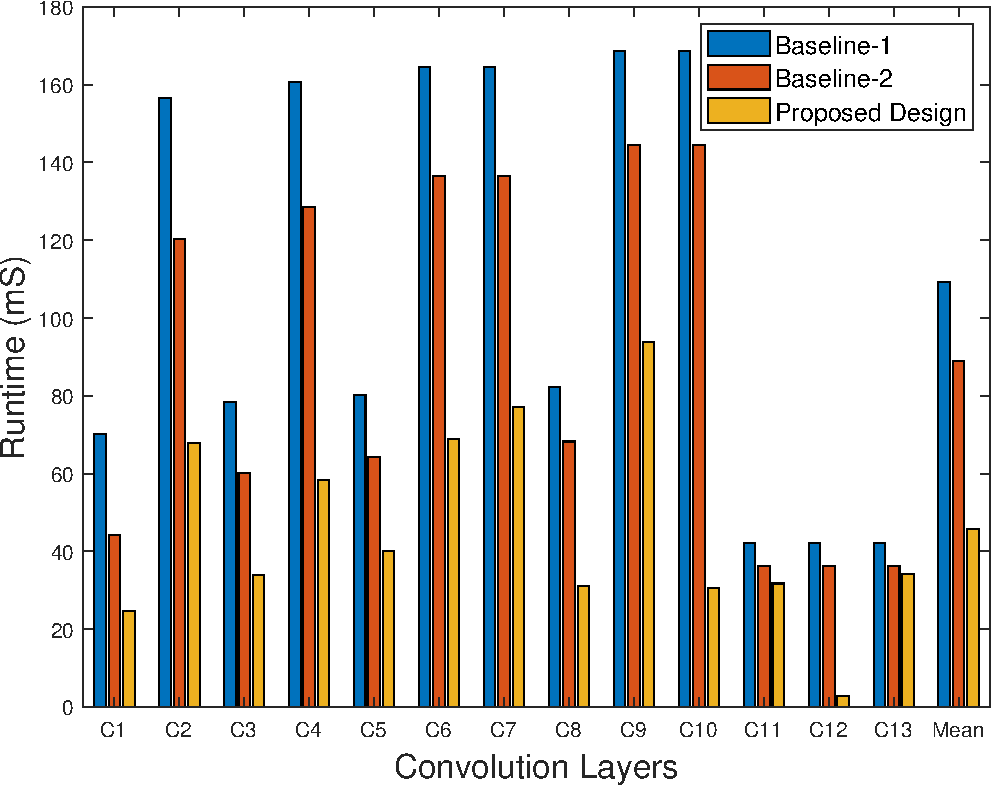
\includegraphics[width=\linewidth]{VGG_duration.pdf}
         \caption{VGG-16}
         \label{fig:runtime_VGG}
     \end{subfigure}
     \hfill
     \begin{subfigure}[b]{\linewidth}
         \centering
         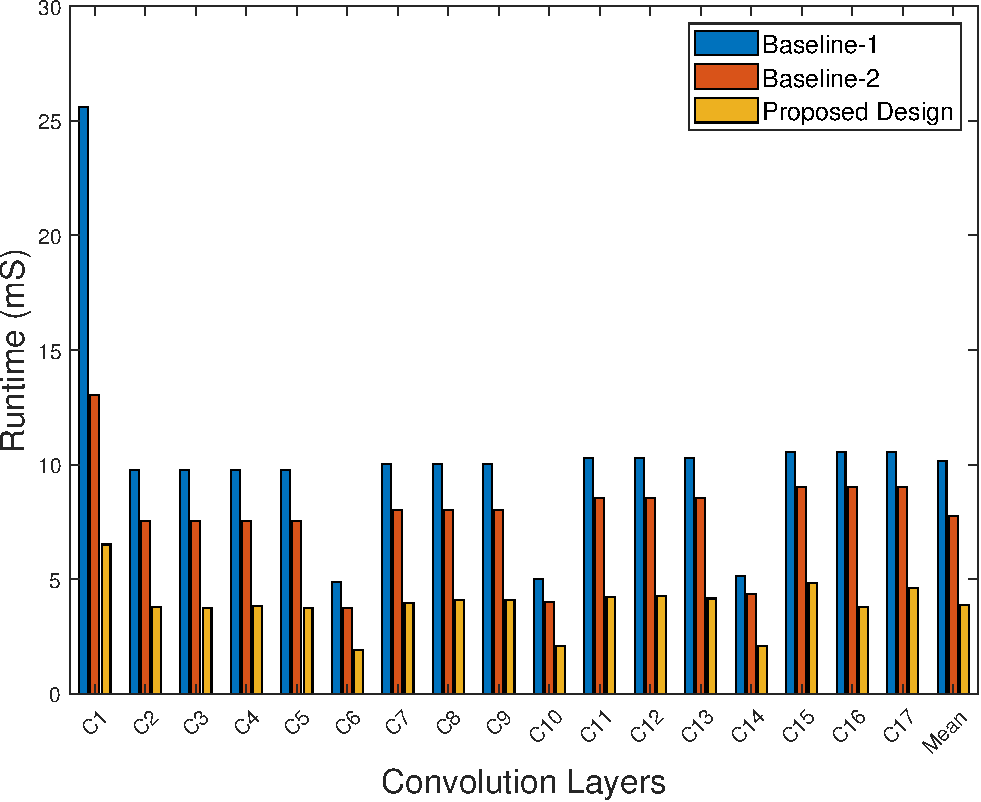
\includegraphics[width=\linewidth]{ResNet_duration.pdf}
         \caption{ResNet-18}
         \label{fig:runtime_ResNet}
     \end{subfigure}
     \caption{Runtimes of the convolution layers for the proposed method with the baseline designs. The proposed design achieved mean runtime improvements of 58.16\% and 61.8\% compared to conventional bit-serial design (Baseline-1) for VGG-16 and ResNet-18 workloads respectively.}
     \label{fig:runtimes}
\end{figure}

Fig.~\ref{fig:runtimes} presents the runtimes of the proposed design compared to the baseline methods. From the figures, it can be noted that the accelerator design based on online arithmetic (Baseline-2) outperforms the conventional bit-serial design (Baseline-1) even without the capability of early detection of the negative outputs, which emphasizes the superiority of the online arithmetic-based designs over the conventional bit-serial designs. As shown in Fig.~\ref{fig:runtime_VGG}, the proposed design showcases mean improvements of 58.16\% and 48.57\% in runtime compared to Baseline-1 and Baseline-2 designs respectively, for the VGG-16 workloads. Similarly, as shown in Fig.~\ref{fig:runtime_ResNet}, the proposed design achieves 61.8\% and 50.15\% respective improvements in runtime on ResNet-18 workloads. These average runtime improvements lead to avergae speedups of \(2.39\times\) and \(2.62\times\) for VGG-16 and ResNet-18 CNN models, respectively, compared to conventional bit-serial design. Similarly, compared to online arihtmetic-based design without the capability of early detection and termination of negative outputs, the proposed design achieves an average speedup of \(1.9\times\) and \(2.01\times\) for VGG-16 and ResNet-18 workloads, respectively. The faster runtimes of the proposed design do not only result due to the efficient design of the online arithmetic-based processing elements, but also due to the large number of negative output activations which in-turn helps in terminating the ineffectual computations resulting is substantial power savings.

\begin{figure}
     \centering
     \begin{subfigure}[b]{\linewidth}
         \centering
         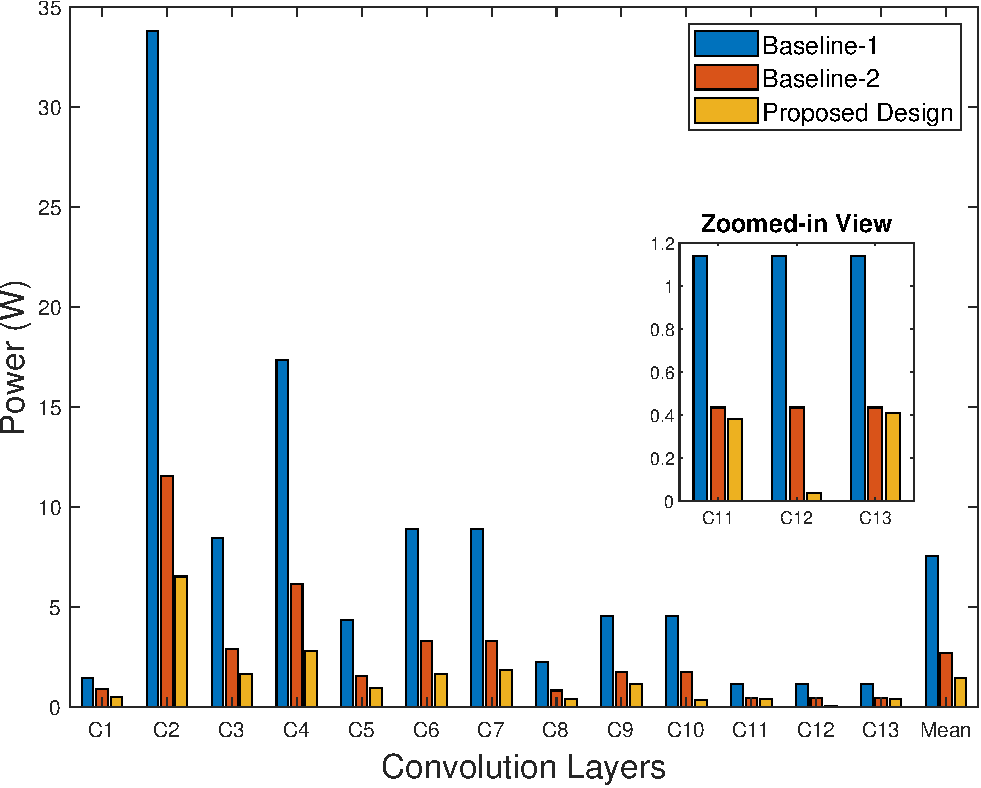
\includegraphics[width=\linewidth]{VGG_power.pdf}
         \caption{VGG-16}
         \label{fig:power_VGG}
     \end{subfigure}
     \hfill
     \begin{subfigure}[b]{\linewidth}
         \centering
         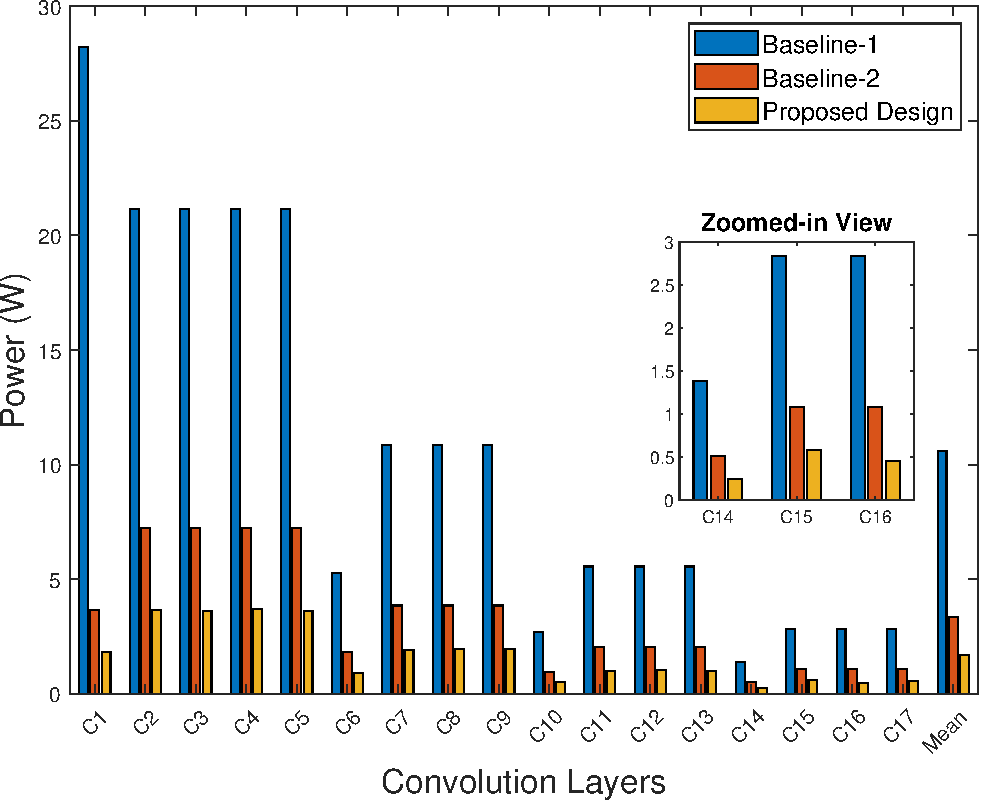
\includegraphics[width=\linewidth]{ResNet_power.pdf}
         \caption{ResNet-18}
         \label{fig:power_ResNet}
     \end{subfigure}
     \caption{Power consumption of the proposed design with the baseline designs. The proposed design achieved 81\% and 84.15\% mean reduction in power consumption compared to conventional bit-serial design (Baseline-1) for VGG-16 and ResNet-18 workloads respectively.}
     \label{fig:power_consumption}
\end{figure}

The power consumption is related to the execution time as well as the utilization of resources in the accelerator. The proposed early detection and termination of negative output activations can result in substantial improvements in power consumption. Fig.~\ref{fig:power_consumption} shows the layer-wise power consumption of the proposed design compared to the baseline designs. For VGG-16 model, as shown in Fig.~\ref{fig:power_VGG}, the proposed design achieves 81\% and 47.16\% improvements in power consumption compared to Baseline-1 and Baseline-2 designs respectively. Similarly, as depicted in Fig.~\ref{fig:power_ResNet}, the proposed design shows significant improvements of 84.15\% and 49.8\% in power consumption for ResNet-18 workloads compared to Baseline-1 and Baseline-2 designs respectively. 




\section{Conclusion} \label{sec: Conclusion}
\textcolor{red}{In this paper we presented DSLOT-NN which utilize online arithmetic based arithmetic operators for the acceleration of  convolution layers in deep neural networks. The online arithmetic presents various benefits including shorter latency, variable precision and digit-level pipelining. We implemented a mechanism to detect and terminate the ineffective convolutions which resulted in power savings and increased performance. In particular, the proposed design has approximately $50\%$ higher performance compared to the state-of-the-art approach for convolution computation. In future, we plan to analyze the behavior of online arithmetic in DNN acceleration with variable input and kernel precision in an inter-layer as well as intra-layer setting. Furthermore, the sparsity in the input and kernels will also be exploited to further improve the performance and energy efficiency of the proposed design.}

% \section{Acknowledgements}
% This research was supported by Basic Science Research Program funded by the Ministry of Education through the National Research Foundation of Korea (NRF-2020R1I1A3063857). We also acknowledge the "HPC Support" Project, supported by the ‘Ministry of Science and ICT’ and NIPA in Korea. The EDA tool was supported by the IC Design Education Center (IDEC), Korea.









\bibliographystyle{IEEEtran}
\bibliography{ref.bib}
\vspace{12pt}


\end{document}
